\DontFrameThisInToc
\Annex{Implémentations du \texttt{Clustering Interactif}}
\label{annex:C-ANNEXE-IMPLEMENTATIONS}

	% INTRODUCTION : annoncer 3 librairies.
	Au cours de ce doctorat, nous avons réalisé un ensemble d'implémentations en \texttt{Python} afin de mettre en oeuvre notre méthodologie de \texttt{Clustering Interactif}.
	Cette implémentation est répartie en trois librairies :
	\begin{enumerate}
		% cognitivefactory-interactive-clustering
		\item \texttt{cognitivefactory-interactive-clustering} \footnote{
			\url{https://pypi.org/project/cognitivefactory-interactive-clustering/}
		} (\cite{schild:2022:cognitivefactory-interactiveclustering}), regroupant les gestions de données et des contraintes, les algorithmes de \textit{clustering} et d'échantillonnage ;
		% cognitivefactory-interactive-clustering-gui
		\item \texttt{cognitivefactory-interactive-clustering-gui} \footnote{
			\url{https://pypi.org/project/cognitivefactory-interactive-clustering-gui/}
		} (\cite{schild-etal:2022:cognitivefactory-interactiveclusteringgui}), intégrant la logique de la méthodologie dans une application web ;
		% cognitivefactory-features-maximization-metric
		\item \texttt{cognitivefactory-features-maximization-metric} \footnote{
			\url{https://pypi.org/project/cognitivefactory-features-maximization-metric/}
		} (\cite{schild:2023:cognitivefactory-featuresmaximizationmetric}), disposant d'une méthode de sélection des patterns linguistiques caractéristiques d'un jeu de données labellisées, permettant ainsi d'analyser la pertinence d'un résultat de \textit{clustering} en fonction du vocabulaire utilisé dans chaque \textit{cluster}.
	\end{enumerate}
	
	%Information : Développements Python.
	\setcounter{localCounterOfFootnoteValue}{\value{footnote}}
	\begin{leftBarInformation}
		Ces implémentations sont disponibles sur le GitHub \url{https://github.com/cognitivefactory}.
		Les \textit{pipelines} d'intégration continue contiennent les étapes
		% Vérification formatage.
		de formatage du code (\textit{grâce aux librairies \texttt{isort} \footnotemark et \texttt{black} \footnotemark}),
		% Vérification qualité et typage.
		de vérification de la qualité et du typage du code (\textit{grâce aux librairies \texttt{flake8} \footnotemark et \texttt{mypy} \footnotemark}),
		% Vérification vulnérabilités.
		de la vérification des vulnérabilités et des failles de sécurité (\textit{grâce à la librairie \texttt{safety} \footnotemark}),
		% Vérification tests unitaires.
		de l'exécution de tests unitaires et de la vérification de la couverture du code testé (\textit{grâce aux librairies \texttt{pytest} \footnotemark et \texttt{coverage} \footnotemark}),
		% Vérification documentation.
		et de la génération de la documentation technique (\textit{grâce à la librairie \texttt{mkdocs} \footnotemark}).
	\end{leftBarInformation}
	% Rattraper les footnote.
		\stepcounter{localCounterOfFootnoteValue}
		\footnotetext[\value{localCounterOfFootnoteValue}]{
			\url{https://pypi.org/project/isort/}
		}
		\stepcounter{localCounterOfFootnoteValue}
		\footnotetext[\value{localCounterOfFootnoteValue}]{
			\url{https://pypi.org/project/black/}
		}
		\stepcounter{localCounterOfFootnoteValue}
		\footnotetext[\value{localCounterOfFootnoteValue}]{
			\url{https://pypi.org/project/flake8/}
		}
		\stepcounter{localCounterOfFootnoteValue}
		\footnotetext[\value{localCounterOfFootnoteValue}]{
			\url{https://pypi.org/project/mypy/}
		}
		\stepcounter{localCounterOfFootnoteValue}
		\footnotetext[\value{localCounterOfFootnoteValue}]{
			\url{https://pypi.org/project/safety/}
		}
		\stepcounter{localCounterOfFootnoteValue}
		\footnotetext[\value{localCounterOfFootnoteValue}]{
			\url{https://pypi.org/project/pytest/}
		}
		\stepcounter{localCounterOfFootnoteValue}
		\footnotetext[\value{localCounterOfFootnoteValue}]{
			\url{https://pypi.org/project/coverage/}
		}
		\stepcounter{localCounterOfFootnoteValue}
		\footnotetext[\value{localCounterOfFootnoteValue}]{
			\url{https://pypi.org/project/mkdocs/}
		}
	
	Dans cette annexe, nous allons détailler ces implémentations, leurs fonctionnalités et certains des choix de mises en oeuvres.
	
	
	% TABLE DES MATIÈRES DE L'ANNEXE.
	\minitoc
	
	
	%%%%%--------------------------------------------------------------------
	%%%%% Section C.1: Implémentation de la librairie \texttt{cognitivefactory-interactive-clustering}
	%%%%%--------------------------------------------------------------------
	\newpage
	\section[
		\texttt{cognitivefactory-interactive-clustering}
	]{
		Implémentation de la librairie \\ \texttt{cognitivefactory-interactive-clustering}
	}
\label{annex:C.1-DESCRIPTION-IMPLEMENTATION-INTERACTIVE-CLUSTERING}
	
	% Généralités.
	La librairie \texttt{cognitivefactory-interactive-clustering} \footnote{
		\url{https://pypi.org/project/cognitivefactory-interactive-clustering/}
	} (\cite{schild:2022:cognitivefactory-interactiveclustering}) a été implémentée au cours de ce doctorat dans le but de mettre à disposition un ensemble d'algorithmes nécessaires à l'utilisation de notre méthodologie de \texttt{Clustering Interactif}.
	Cette librairie comporte plusieurs fonctionnalités :
	\begin{itemize}
		\item la gestion des données avec leurs prétraitements et leur vectorisation (cf. \textsc{Section~\ref{annex:C.1.1-DESCRIPTION-IMPLEMENTATION-INTERACTIVE-CLUSTERING-GESTION-DES-DONNEES}}) ;
		\item la gestion des contraintes avec le calcul des propriétés de transitivité et la détection des conflits (cf. \textsc{Section~\ref{annex:C.1.2-DESCRIPTION-IMPLEMENTATION-INTERACTIVE-CLUSTERING-GESTION-DES-CONTRAINTES}}) ;
		\item l'exécution d'algorithmes de \textit{clustering} sous contraintes pour proposer une segmentation des données (cf. \textsc{Section~\ref{annex:C.1.3-DESCRIPTION-IMPLEMENTATION-INTERACTIVE-CLUSTERING-ALGORITHMES-CLUSTERING-SOUS-CONTRAINTES}}) ;
		\item l'exécution d'algorithmes d'échantillonnage pour sélectionner les prochaines contraintes à annoter (cf. \textsc{Section~\ref{annex:C.1.4-DESCRIPTION-IMPLEMENTATION-INTERACTIVE-CLUSTERING-ALGORITHMES-ECHANTILLONNAGE-DE-CONTRAINTES}}).
	\end{itemize}
	
	Nous présentons succinctement cette librairie avec certains choix d'implémentation.
	
	% Information : comme y accéder.
	\begin{leftBarInformation}
		La documentation technique de cette librairie est accessible par le lien suivant : \url{https://cognitivefactory.github.io/interactive-clustering/}.
	\end{leftBarInformation}
	
	% Exemple.
	Pour les sections suivantes, nous suivrons l'exemple suivant (cf. \textsc{Code~\ref{code:C.1-DESCRIPTION-IMPLEMENTATION-INTERACTIVE-CLUSTERING-DATA}}) pour présenter nos implémentations.
	
	\begin{lstlisting}[
		language=Python,
		caption={Jeu exemple pour présenter notre implémentation du \texttt{Clustering Interactif}.},
		label={code:C.1-DESCRIPTION-IMPLEMENTATION-INTERACTIVE-CLUSTERING-DATA},
	]
# Définir les données.
dict_of_texts = {
	"0": "Comment signaler un vol de carte bancaire ?",
	"1": "J'ai égaré ma carte bancaire, que faire ?",
	"2": "J'ai perdu ma carte de paiement",
	"3": "Le distributeur a avalé ma carte !",
	"4": "En retirant de l'argent, le GAB a gardé ma carte...",
	"5": "Le distributeur ne m'a pas rendu ma carte bleue.",
	# ...
	"N": "Pourquoi le sans contact ne fonctionne pas ?",
}
	\end{lstlisting}
	
	
	%%%
	%%% Subsection C.1.1: Gestion des données.
	%%%
	\subsection{Gestion des données}
	\label{annex:C.1.1-DESCRIPTION-IMPLEMENTATION-INTERACTIVE-CLUSTERING-GESTION-DES-DONNEES}
	
	% cognitivefactory.interactive-clustering.utils
	Tout d'abord, en ce qui concerne la \textbf{manipulation de données}, nous utilisons le module \texttt{utils} de la librairie \texttt{cognitivefactory-interactive-clustering}.
	Les données sont stockées dans un dictionnaire \texttt{Python} afin de tracer les manipulations à l'aide d'une clé servant d'identifiant de la donnée.
	
	% cognitivefactory.interactive-clustering.utils.preprocessing : Implémentation.
	Nous avons d'une part la partie \texttt{utils.preprocessing} \footnote{
		\url{https://cognitivefactory.github.io/interactive-clustering/reference/cognitivefactory/interactive_clustering/utils/preprocessing/}
	} qui permet de normaliser les données.
	Par défaut :
	\begin{itemize}
		\item[\(\bullet\)] le texte est passé en \textit{minuscule} (de \textguillemets{\texttt{Bonjour}} à \textguillemets{\texttt{bonjour}}),
		\item[\(\bullet\)] la \textit{ponctuation} est supprimée \textguillemets{\texttt{c'est-à-dire ?!}} à \textguillemets{\texttt{c est a dire}}), %(\texttt{.}, \texttt{,}, \texttt{;}, \texttt{:}, \texttt{!}, \texttt{¡}, \texttt{?}, \texttt{¿}, \texttt{…}, \texttt{•}, \texttt{(}, \texttt{)}, \texttt{\{}, \texttt{\}}, \texttt{[}, \texttt{]}, \texttt{\textguillemets{}, \texttt{}}, \texttt{^}, \texttt{\`}, \texttt{'}, \texttt{"}, \texttt{\\}, \texttt{/}, \texttt{|}, \texttt{-}, \texttt{\_}, \texttt{#}, \texttt{\&}, \texttt{\~}, \texttt{\@}),
		\item[\(\bullet\)] les \textit{accents} sont enlevés (de \textguillemets{\texttt{crédit}} à \textguillemets{\texttt{credit}}),
		\item[\(\bullet\)] et les multiples \textit{espaces blancs} sont convertis en un unique espace simple (de \textguillemets{\texttt{au~~~~revoir}} à \textguillemets{\texttt{au revoir}}).
	\end{itemize}
	
	Si besoin, trois options "avancées" sont disponibles pour réaliser des prétraitements plus destructifs :
	\begin{itemize}
		\item[\(\bullet\)] la suppression des mots vides (\textit{stopwords}, \cite{nothman-etal:2018:stop-word-lists}),
		\item[\(\bullet\)] la conversion des mots vers leur forme racine (\textit{lemmatisation}, \cite{manning-schutze:2000:foundations-statistical-natural}),
		\item[\(\bullet\)] et la suppression des mots en fonction de leur profondeur dans l'arbre de dépendances syntaxiques (\cite{nivre:2006:inductive-dependency-parsing}).
	\end{itemize}
	
	% cognitivefactory.interactive-clustering.utils.preprocessing : Dépendances.
	Ces traitements sont réalisés en bénéficiant des fonctionnalités mises à disposition d'un modèle de langue de type SpaCy (\cite{honnibal-montani:2017:spacy-natural-language}), avec par défaut l'utilisation du modèle \texttt{fr-core-news-md}.
	
	% cognitivefactory.interactive-clustering.utils.preprocessing : Par défaut.
	Pour nos études, nous définissons quatre niveaux de prétraitements facilement identifiables :
	\begin{enumerate}
		\item L'\textbf{absence de prétraitements}, soit la conservation de la donnée brute, noté \texttt{prep.no} ;
		\item Les \textbf{prétraitements simples}, correspondant au traitement de base (minuscules, ponctuations, accents, espaces blancs), notés \texttt{prep.simple} ; 
		\item Les \textbf{prétraitements avec lemmatisation}, correspondant au traitement de base auquel s'ajoute la conversion des mots vers leur forme racine, notés \texttt{prep.lemma} ;
		\item les \textbf{prétraitements avec filtres}, correspondant au traitement de base avec l'élagage de l'arbre de dépendance syntaxique de la phrase, notés \texttt{prep.filter}.
	\end{enumerate}
	
	
	% cognitivefactory.interactive-clustering.utils.vectorization
	D'autre part, la partie \texttt{utils.vectorization} \footnote{
		\url{https://cognitivefactory.github.io/interactive-clustering/reference/cognitivefactory/interactive_clustering/utils/vectorization/}
	} permet de transformer les données en une représentation exploitable pour la machine.
	Deux modes de vectorisation sont mis à disposition :
	\begin{enumerate}
		\item \textbf{TF-IDF} (\cite{ramos:2003:using-tfidf-determine}), utilisant la fréquence d'occurrence des mots pour représenter une phrase, et noté \texttt{vect.tfidf} pour nos études ;
		\item \textbf{SpaCy} (\cite{honnibal-montani:2017:spacy-natural-language}), utilisant le modèle de langue \texttt{fr-core-news-md}, et noté \texttt{vect.frcorenewsmd}.
	\end{enumerate}
	
	% cognitivefactory.interactive-clustering.utils : Exemple.
	Vous avez un exemple d'utilisation des modules de prétraitements et de vectorisation dans \textsc{Code~\ref{code:C.1.1-DESCRIPTION-IMPLEMENTATION-INTERACTIVE-CLUSTERING-GESTION-DONNEES}}.
	
	\begin{lstlisting}[
		language=Python,
		caption={Démonstration de notre implémentation des prétraitements et de la vectorisation sur le jeu d'exemples.},
		label={code:C.1.1-DESCRIPTION-IMPLEMENTATION-INTERACTIVE-CLUSTERING-GESTION-DONNEES},
	]
# Import des dépendances.
from cognitivefactory.interactive_clustering.utils.preprocessing import preprocess
from cognitivefactory.interactive_clustering.utils.vectorization import vectorize

# Prétraitement des données.
dict_of_preprocess_texts = preprocess(
	dict_of_texts=dict_of_texts,
	apply_stopwords_deletion=False,
	apply_parsing_filter=False,
	apply_lemmatization=False,
	spacy_language_model="fr_core_news_md",
)
"""
{"0": "comment signaler un vol de carte bancaire",
 "1": "j ai egare ma carte bancaire, que faire",
 "2": "j ai perdu ma carte de paiement",
 "3": "le distributeur a avale ma carte",
 "4": "en retirant de l argent le gab a garde ma carte",
 "5": "le distributeur ne m a pas rendu ma carte bleue",
 # ...
 "N": "pourquoi le sans contact ne fonctionne pas"}
"""

# Vectorisation des données.
dict_of_vectors = vectorize(
	dict_of_texts=dict_of_preprocess_texts,
	vectorizer_type="tfidf",
)
	\end{lstlisting}
	
	%%%
	%%% Subsection C.1.2: Gestion des contraintes
	%%%
	\subsection{Gestion des contraintes}
	\label{annex:C.1.2-DESCRIPTION-IMPLEMENTATION-INTERACTIVE-CLUSTERING-GESTION-DES-CONTRAINTES}
	
	% cognitivefactory.interactive-clustering.constraints
	En ce qui concerne la \textbf{manipulation de contraintes}, nous utilisons le module \texttt{contraints} \footnote{
		\url{https://cognitivefactory.github.io/interactive-clustering/reference/cognitivefactory/interactive_clustering/constraints/}
	} de la librairie \texttt{cognitivefactory-interactive-clustering}.
	
	% cognitivefactory.interactive-clustering.constraints: Types
	Deux types de contraintes sont prises en charge (cf. \cite{wagstaff-cardie:2000:clustering-instancelevel-constraints}) :
	\begin{itemize}
		\item[\(\bullet\)] les contraintes \texttt{MUST-LINK} permettant de réunir deux données,
		\item[\(\bullet\)] et les contraintes \texttt{CANNOT-LINK} permettant à l'inverse de les séparer.
	\end{itemize}

	% cognitivefactory.interactive-clustering.constraints: Transitivité.
	Ces types de contraintes respectent les propriétés de transitivité décrites dans l'\textsc{Equation~\ref{equation:C.1.2-DESCRIPTION-IMPLEMENTATION-INTERACTIVE-CLUSTERING-CONTRAINTES-TRANSITIVITE}}) et sont illustrées dans la \textsc{Figure~\ref{figure:C.1.2-DESCRIPTION-IMPLEMENTATION-INTERACTIVE-CLUSTERING-CONTRAINTES-TRANSITIVITE}} (\textbf{(1)} et \textbf{(2)}).
	Nous notons ainsi qu'il est possible de déduire la troisième contrainte d'un triangle de trois points si nous connaissons déjà les deux premières.
	
	\begin{equation}
		\label{equation:C.1.2-DESCRIPTION-IMPLEMENTATION-INTERACTIVE-CLUSTERING-CONTRAINTES-TRANSITIVITE}
		(\forall A,B,C)~
		\begin{cases}
			% ML + ML => ML
			~\textcolor{colorDarkPastelGreen}{\texttt{MUST\_LINK}}(A,B)
			~\wedge~\textcolor{colorDarkPastelGreen}{\texttt{MUST\_LINK}}(B,C)
			~\Rightarrow~\textcolor{colorDarkPastelGreen}{\texttt{MUST\_LINK}}(A,C)  \\
			% ML + CL => CL
			~\textcolor{colorDarkPastelGreen}{\texttt{MUST\_LINK}}(A,B)
			~\wedge~\textcolor{colorDarkPastelRed}{\texttt{CANNOT\_LINK}}(B,C)
			~\Rightarrow~\textcolor{colorDarkPastelRed}{\texttt{CANNOT\_LINK}}(A,C)
		\end{cases}
	\end{equation}
	
	Pour respecter ces propriétés, le gestionnaire de contraintes doit calculer les transitivités à chaque ajout ou suppression de contraintes.
	Nous distinguerons donc une contrainte ajoutée (\texttt{added}) d'une contrainte déduite par transitivité (\texttt{inferred}).
	
	% cognitivefactory.interactive-clustering.constraints: Conflits.
	Il se peut que la contrainte en cours d'ajout contredise les contraintes précédemment déduites : nous parlons alors d'incohérence ou de conflit (cf. \textsc{Figure~\ref{figure:C.1.2-DESCRIPTION-IMPLEMENTATION-INTERACTIVE-CLUSTERING-CONTRAINTES-TRANSITIVITE}} et \textsc{Equation~\ref{equation:C.1.2-DESCRIPTION-IMPLEMENTATION-INTERACTIVE-CLUSTERING-CONTRAINTES-CONFLITS}}).
	Dans ce cas, l'ajout de la dernière contrainte n'est pas pris en compte et le gestionnaire renvoie une erreur permettant d'identifier ce conflit.
	Ce conflit peut simplement venir d'une erreur d'inattention, mais peut aussi venir d'une déduction basée sur des ajouts antérieurs erronés.
	Sémantiquement, un conflit indique une contradiction dans la gestion des données, dû au fait que les données concernées doivent à la fois être réunies et séparées...
	
	\begin{equation}
		\label{equation:C.1.2-DESCRIPTION-IMPLEMENTATION-INTERACTIVE-CLUSTERING-CONTRAINTES-CONFLITS}
		(\exists A,B,C)~
		~\textcolor{colorDarkPastelGreen}{\texttt{MUST\_LINK}}(A,B)
		~\wedge~\textcolor{colorDarkPastelGreen}{\texttt{MUST\_LINK}}(B,C)
		~\wedge~\textcolor{colorDarkPastelRed}{\texttt{CANNOT\_LINK}}(A,C)
	\end{equation}
	
	% cognitivefactory.interactive-clustering.constraints: Composants connexe.
	À partir d'une donnée \(D\), et par application de la propriété de transitivité des \texttt{MUST-LINK}, nous appelons \textbf{composant connexe} de \(D\) l'ensemble des données \(D_i\) liées par une succession de contraintes \texttt{MUST-LINK} à \(D\) (cf. \textsc{Figure~\ref{figure:C.1.2-DESCRIPTION-IMPLEMENTATION-INTERACTIVE-CLUSTERING-CONTRAINTES-TRANSITIVITE}}).
	Ce composant peut être vu comme un noyau de \textit{clusters}.
	Il pourra être associé à d'autres noyaux par similarité pour former un \textit{cluster} plus conséquent, ou être distingué d'autres noyaux pour former plusieurs \textit{clusters}.

	\begin{figure}[!htb]
		\centering
		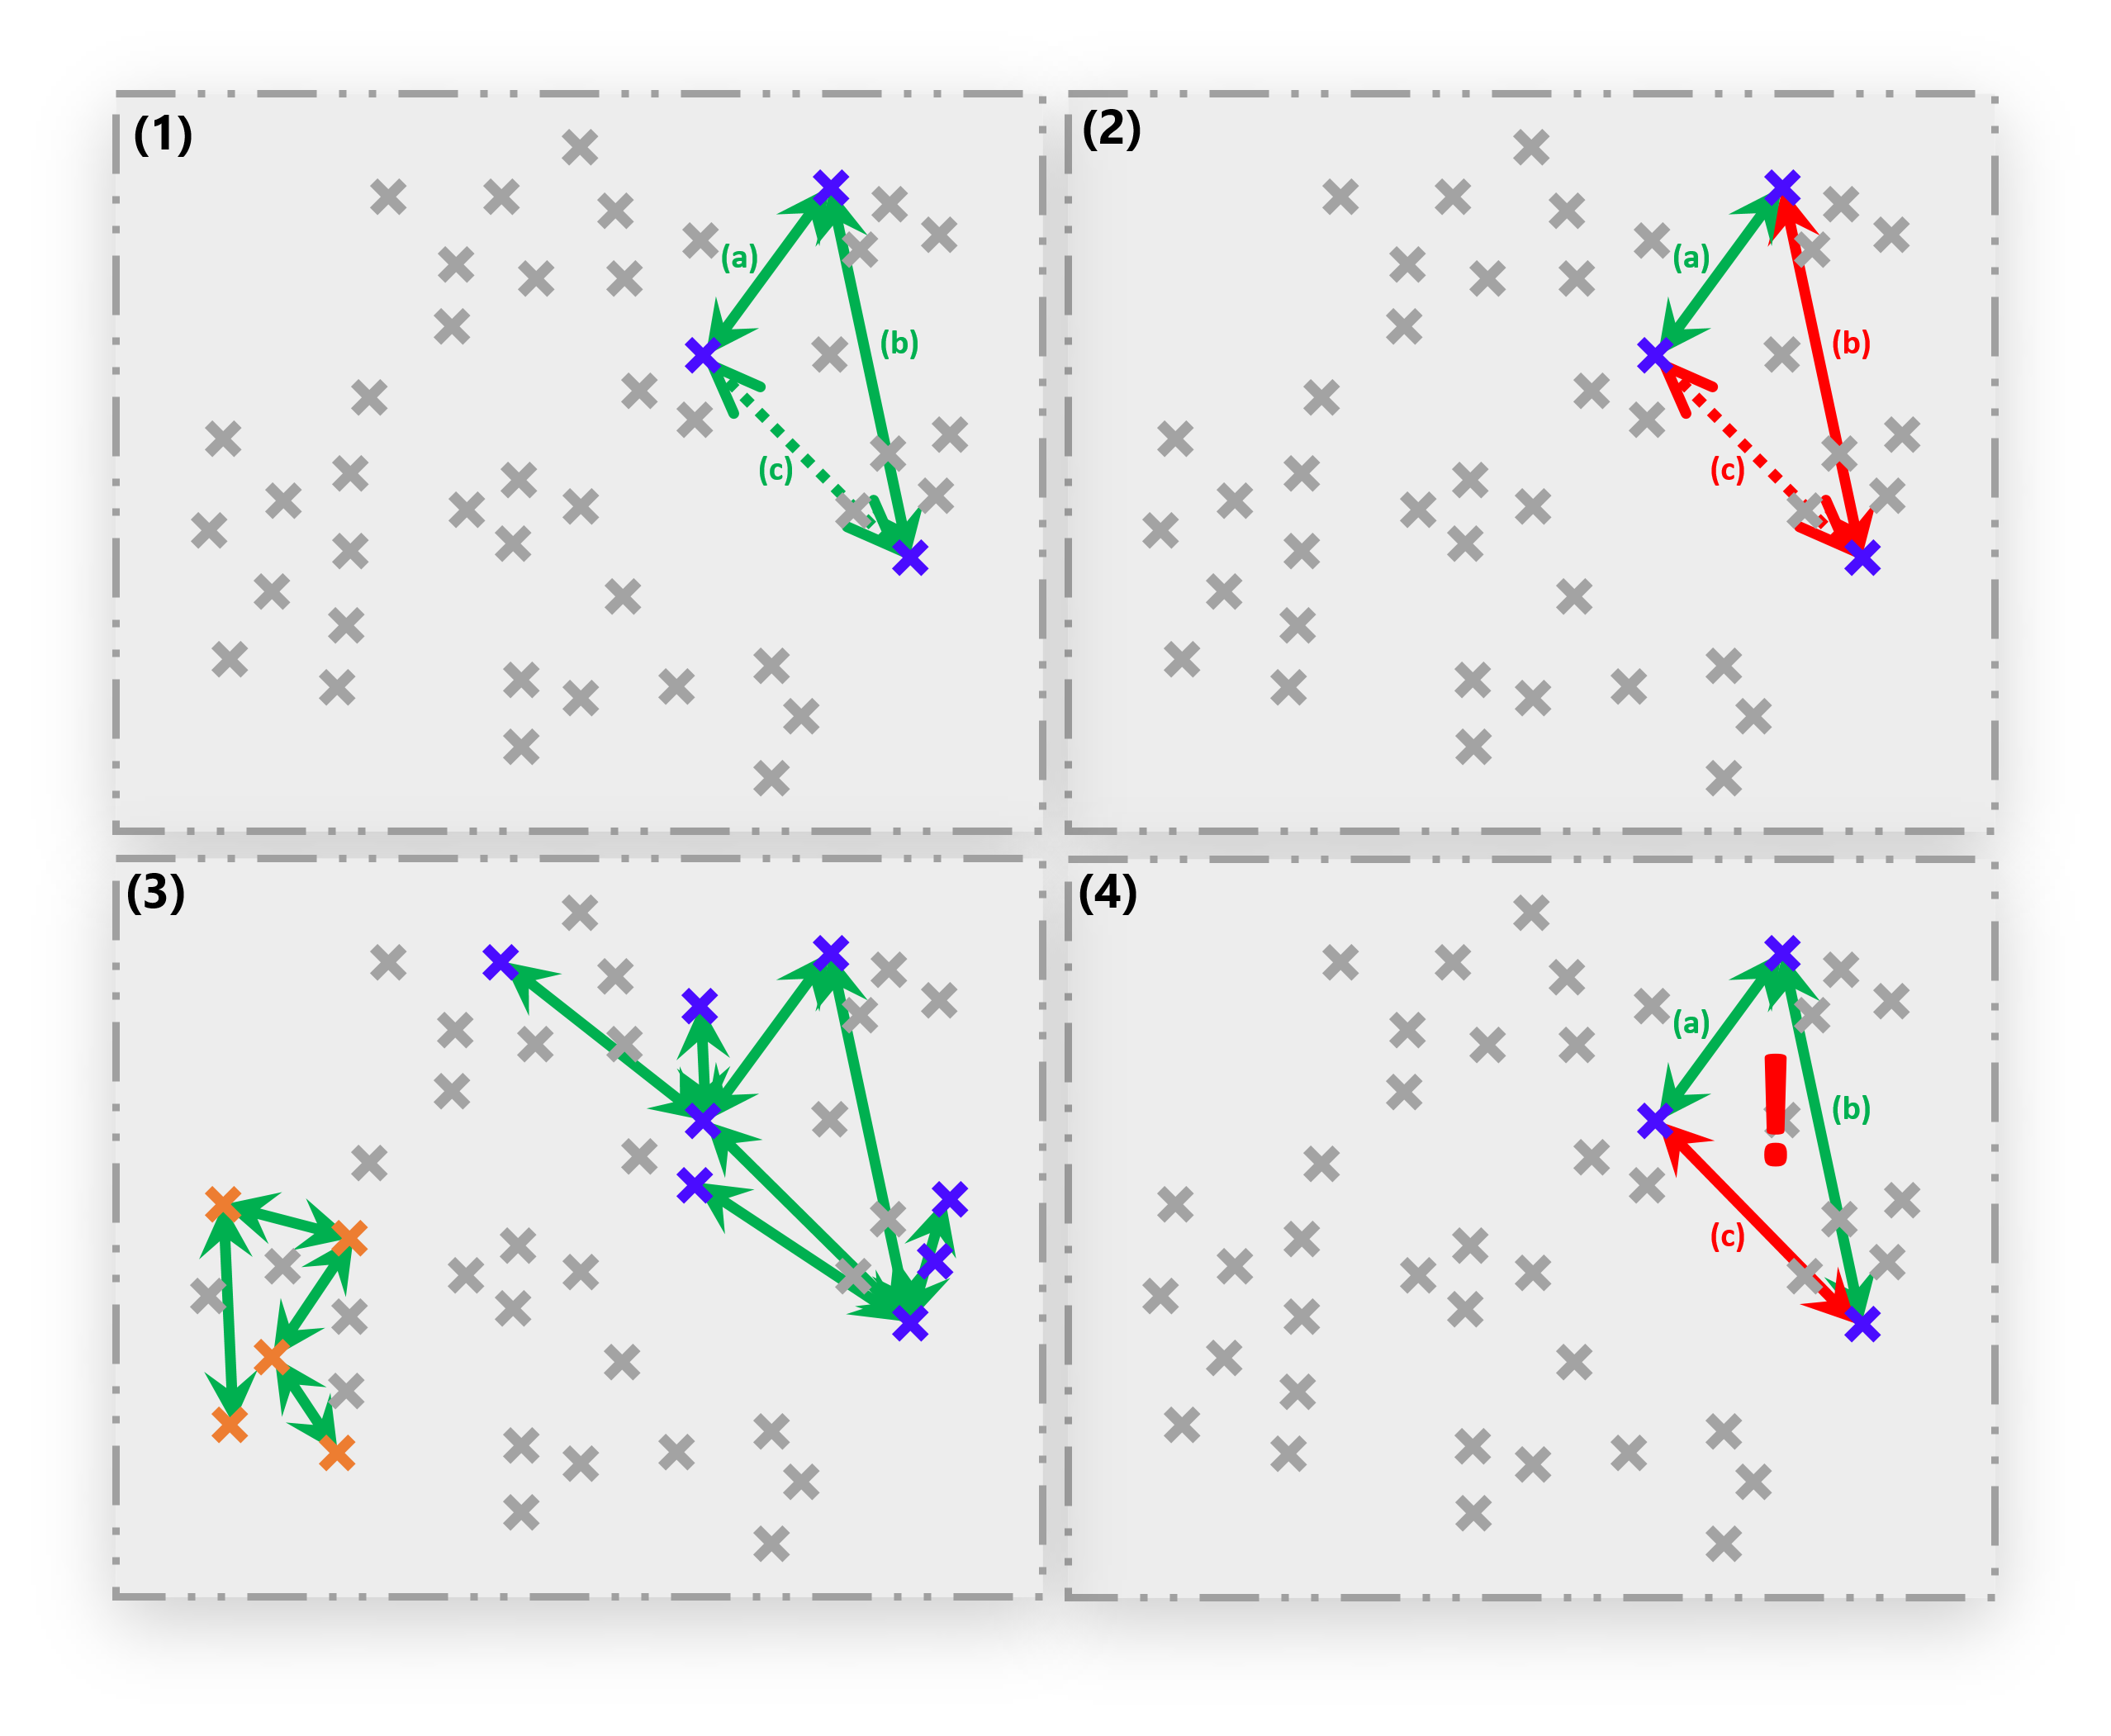
\includegraphics[width=0.70\textwidth]{figures/example-constraints-transitivity}
		\caption{
			Exemples des propriétés de transitivité des contraintes \texttt{MUST-LINK} (flèches vertes) et \texttt{CANNOT-LINK} (flèches rouges). \textbf{(1)} et \textbf{(2)} représentent les possibilités de déduction d'une contrainte (\texttt{(c)}) en fonction des deux autres (\texttt{(a)} et \texttt{(b)}). \textbf{(3)} représente deux composants connexes définis par la transitivité des contraintes \texttt{MUST-LINK}. Enfin, \textbf{(4)} représente un cas de conflit où une contrainte (\texttt{(c)}) ne correspond pas à sa déduction faite à partir des autres contraintes (\texttt{(a)} et \texttt{(b)}).
		}
		\label{figure:C.1.2-DESCRIPTION-IMPLEMENTATION-INTERACTIVE-CLUSTERING-CONTRAINTES-TRANSITIVITE}
	\end{figure}
	
	% cognitivefactory.interactive-clustering.constraints : Exemple.
	Un exemple d'utilisation du module de gestion de contraintes est consultable dans \textsc{Code~\ref{code:C.1.2-DESCRIPTION-IMPLEMENTATION-INTERACTIVE-CLUSTERING-GESTION-CONTRAINTES}}.
	
	\begin{lstlisting}[
		language=Python,
		caption={Démonstration de notre implémentation de gestion des contraintes sur le jeu d'exemples.},
		label={code:C.1.2-DESCRIPTION-IMPLEMENTATION-INTERACTIVE-CLUSTERING-GESTION-CONTRAINTES},
	]
# Import des dépendances.
from cognitivefactory.interactive_clustering.constraints.factory import managing_factory

# Création du gestionnaire de contraintes.
constraints_manager = managing_factory(
	manager="binary",
	list_of_data_IDs = list(dict_of_texts.keys()),
	# ["0", "1", "2", "3", "4", "5", ..., "N"]
)

# Ajout de contraintes.
constraints_manager.add_constraint(
	data_ID1="0",  # "Comment signaler un vol de carte bancaire ?"
	data_ID2="1",  # "J'ai égaré ma carte bancaire, que faire ?"
	constraint_type="MUST_LINK",
)
constraints_manager.add_constraint(
	data_ID1="3",  # "Le distributeur a avalé ma carte !"
	data_ID2="4",  # "En retirant de l'argent, le GAB a gardé ma carte..."
	constraint_type="MUST_LINK",
)
constraints_manager.add_constraint(
	data_ID1="0",  # "Comment signaler un vol de carte bancaire ?"
	data_ID2="N",  # "Pourquoi le sans contact ne fonctionne pas ?"
	constraint_type="CANNOT_LINK",
)
# NB: ajouter une contrainte "MUST_LINK" entre "1" et "N" lèverait une erreur.

# Récupération des composants connexes.
connected_components = constraints_manager.get_connected_components()
"""
[['0', '1'],
 ['2'],
 ['3', '4'],
 ['5'],
 ['N']]
"""
	\end{lstlisting}
	
	
	%%%
	%%% Subsection C.1.3: Algorithme de \textit{clustering} sous contraintes.
	%%%
	\subsection{Algorithme de \textit{clustering} sous contraintes}
	\label{annex:C.1.3-DESCRIPTION-IMPLEMENTATION-INTERACTIVE-CLUSTERING-ALGORITHMES-CLUSTERING-SOUS-CONTRAINTES}
	
	% cognitivefactory.interactive-clustering.clustering
	En ce qui concerne le \textbf{regroupement automatique} des données par similarité, nous utilisons le module \texttt{clustering} \footnote{
		\url{https://cognitivefactory.github.io/interactive-clustering/reference/cognitivefactory/interactive_clustering/clustering/}
	} de la librairie \texttt{cognitivefactory-interactive-clustering}.
	
	% cognitivefactory.interactive-clustering.utils.clustering : Implémentation.
	Ce module met à disposition cinq algorithmes de \textit{clustering} sous contraintes :
	\begin{enumerate}
		\item \textbf{\texttt{KMeans}}, dans sa version \texttt{COP-KMeans} (\cite{wagstaff-etal:2001:constrained-kmeans-clustering}), noté \texttt{clust.kmeans.cop}, et sa version \texttt{MPC-KMeans} (\cite{khan-etal:2012:multiple-parameter-based}), noté \texttt{clust.kmeans.mpc}) ;
		\item \textbf{\texttt{DBscan}}, dans sa version \texttt{C-DBScan} (\cite{ruiz-etal:2010:densitybased-semisupervised-clustering}), noté \texttt{clust.cdbscan} ;
		\item \textbf{Hiérarchique} (\cite{davidson-ravi:2005:agglomerative-hierarchical-clustering}), avec quatre métriques de distances : \texttt{single} (noté \texttt{clust.hier.sing}), \texttt{complete} (noté \texttt{clust.hier.comp}), \texttt{average} (noté \texttt{clust.hier.avg}) et \texttt{ward} (noté \texttt{clust.hier.ward}) ;
		\item \textbf{Spectral}, dans sa version \texttt{SPEC} (\cite{kamvar-etal:2003:spectral-learning}), noté \texttt{clust.spec} ;
		\item \textbf{Propagation par affinité} (\cite{givoni-frey:2009:semisupervised-affinity-propagation}), noté \texttt{clust.affprop}.
	\end{enumerate}
	
	Une classe abstraite définit les prérequis des algorithmes implémentés (avoir une méthode \texttt{cluster}) et une \textit{factory} est disponible pour instancier rapidement un objet de \textit{clustering}.
	% cognitivefactory.interactive-clustering.clustering : Exemple.
	Enfin, un exemple d'utilisation de ce module est consultable dans \textsc{Code~\ref{code:C.1.3-DESCRIPTION-IMPLEMENTATION-INTERACTIVE-CLUSTERING-CLUSTERING}}.
	
	
	\begin{lstlisting}[
		language=Python,
		caption={Démonstration de notre implémentation du \textit{clustering} sous contraintes sur le jeu d'exemples.},
		label={code:C.1.3-DESCRIPTION-IMPLEMENTATION-INTERACTIVE-CLUSTERING-CLUSTERING},
	]
# Import des dépendances.
from cognitivefactory.interactive_clustering.clustering.factory import clustering_factory

# Initialiser un objet de clustering.
clustering_model = clustering_factory(
	algorithm="kmeans",
	model="COP",
	random_seed=42,
)

# Lancer le clustering.
clustering_result = clustering_model.cluster(
	constraints_manager=constraints_manager,
	nb_clusters=2,
	vectors=dict_of_vectors,
)
"""
{"0": 0,  # "Comment signaler un vol de carte bancaire ?"
 "1": 0,  # "J'ai égaré ma carte bancaire, que faire ?"
 "2": 0,  # "J'ai perdu ma carte de paiement"
 "3": 1,  # "Le distributeur a avalé ma carte !"
 "4": 1,  # "En retirant de l'argent, le GAB a gardé ma carte..."
 "5": 1,  # "Le distributeur ne m'a pas rendu ma carte bleue."
 # ...
 "N": 1}  # "Pourquoi le sans contact ne fonctionne pas ?"
"""
	\end{lstlisting}
	
	% cognitivefactory.interactive-clustering.utils.clustering : Historique.
	\begin{leftBarInformation}
		Dans le cadre d'un projet étudiant avec l'École d'Ingénieurs Télécom Physique Strasbourg (au cours de l'année 2022), les implémentations des algorithmes \texttt{MPC-KMeans}, \texttt{C-DBScan} et de propagation par affinité ont été ajoutées. Les élèves ont conclu ce projet d'extension en suggérant de se concentrer sur l'étude du C-DBScan car les deux autres algorithmes étaient soit trop instables, soit trop gourmand en temps de calcul.
		Les autres algorithmes (\texttt{COP-KMeans}, hiérarchique et spectral) ont été implémentés au début de ce doctorat.
	\end{leftBarInformation}
	
	
	%%%
	%%% Subsection C.1.4: Algorithme d'échantillonnage de contraintes.
	%%%
	\subsection{Algorithme d'échantillonnage de contraintes}
	\label{annex:C.1.4-DESCRIPTION-IMPLEMENTATION-INTERACTIVE-CLUSTERING-ALGORITHMES-ECHANTILLONNAGE-DE-CONTRAINTES}
	
	% cognitivefactory.interactive-clustering.sampling
	En ce qui concerne l'\textbf{échantillonnage} de contraintes à annoter, nous utilisons le module \texttt{sampling} \footnote{
		\url{https://cognitivefactory.github.io/interactive-clustering/reference/cognitivefactory/interactive_clustering/sampling/}
	} de la librairie \texttt{cognitivefactory-interactive-clustering}.
	
	% cognitivefactory.interactive-clustering.utils.sampling : Implémentation.
	Cet échantillonnage correspond à la sélection de couple de données.
	Par défaut, l'échantillonnage est purement aléatoire.
	Cependant, plusieurs options sont disponibles :
	
	\begin{itemize}
		\item[\(\bullet\)] une restriction sur la \textit{distance} pouvant imposer aux données d'être les plus proches ou les plus éloignées du corpus ;
		\item[\(\bullet\)] une restriction sur le \textit{résultat du clustering} pouvant imposer aux données d'être issues d'un même \textit{cluster} ou de \textit{clusters} différents,
		\item[\(\bullet\)] une restriction pour exclure les contraintes \textit{déjà annotées},
		\item[\(\bullet\)] et enfin une restriction pour exclure les contraintes \textit{déjà déduites} par transitivité.
	\end{itemize}
	
	% cognitivefactory.interactive-clustering.utils.sampling : Par défaut.
	Sur cette base, nous définissons quatre niveaux d'échantillonnage facilement identifiables pour nos études :
	\begin{enumerate}
		\item Un échantillonnage \textbf{purement aléatoire}, en excluant toutes les contraintes déjà annotées ou déduites, noté \texttt{samp.random.full} ;
		\item Un échantillonnage \textbf{pseudo-aléatoire} de données issues d'un \textbf{même \textit{cluster}}, en excluant toutes les contraintes déjà annotées ou déduites, noté \texttt{samp.random.same} ;
		\item Un échantillonnage des données issues d'un \textbf{même \textit{cluster}} et étant \textbf{les plus éloignées} les unes des autres, noté \texttt{samp.farhtest.same} (cf. \textsc{Figure~\ref{figure:C.1.4-DESCRIPTION-IMPLEMENTATION-INTERACTIVE-CLUSTERING-CONTRAINTES-SAMPLING}}) ;
		\item Un échantillonnage des données issues de \textbf{\textit{clusters} différents} et étant \textbf{les plus proches} les unes des autres, noté \texttt{samp.closest.diff} (cf. \textsc{Figure~\ref{figure:C.1.4-DESCRIPTION-IMPLEMENTATION-INTERACTIVE-CLUSTERING-CONTRAINTES-SAMPLING}}).
	\end{enumerate}
	
	\begin{figure}[!htb]
		\centering
		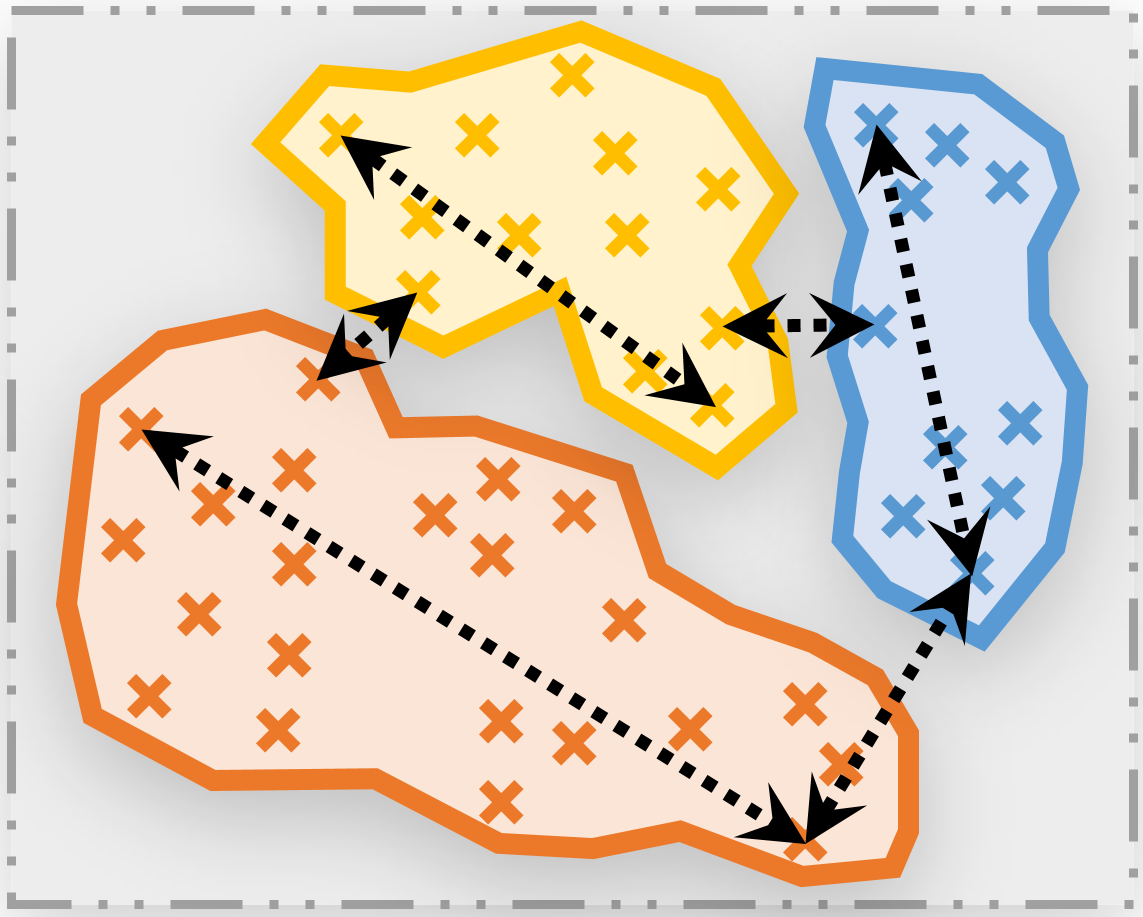
\includegraphics[width=0.35\textwidth]{figures/example-sampling}
		\caption{
			Exemples d'échantillonnages, sur la base de trois clusters, de données issues de mêmes \textit{clusters} et étant les plus éloignées les unes des autres (\texttt{samp.farhtest.same}), et de données issues de clusters différents et étant les plus proches les unes des autres (\texttt{samp.closest.diff}).
		}
		\label{figure:C.1.4-DESCRIPTION-IMPLEMENTATION-INTERACTIVE-CLUSTERING-CONTRAINTES-SAMPLING}
	\end{figure}

	Une classe abstraite définit les prérequis des algorithmes implémentés (avoir une méthode \texttt{sample}) et une \textit{factory} est disponible pour instancier rapidement un objet d'échantillonnage.
	% cognitivefactory.interactive-clustering.sampling : Exemple.
	Un exemple d'utilisation de ce module est consultable dans \textsc{Code~\ref{code:C.1.4-DESCRIPTION-IMPLEMENTATION-INTERACTIVE-CLUSTERING-SAMPLING}}.
	
	\begin{lstlisting}[
		language=Python,
		caption={Démonstration de notre implémentation de l'échantillonnage sur le jeu d'exemples.},
		label={code:C.1.4-DESCRIPTION-IMPLEMENTATION-INTERACTIVE-CLUSTERING-SAMPLING},
	]
# Import des dépendances.
from cognitivefactory.interactive_clustering.sampling.factory import sampling_factory

# Initialiser un objet d'échantillonnage.
sampler = sampling_factory(
	algorithm="random",
	random_seed=42,
)

# Run sampling.
selection = sampler.sample(
	constraints_manager=constraints_manager,
	nb_to_select=2,
	clustering_result=clustering_result,  # optionnel
	vectors=dict_of_vectors,  # optionnel
)
"""
[("0", '5"),  # "Comment signaler un vol de carte bancaire ?" vs "Le distributeur ne m'a pas rendu ma carte bleue."
 ("0", '2"),  # "Comment signaler un vol de carte bancaire ?" vs "J'ai perdu ma carte de paiement"
 ("2", 'N")]  # "J'ai perdu ma carte de paiement" vs "Pourquoi le sans contact ne fonctionne pas ?"
"""
	\end{lstlisting}
	
	
	%%%%%--------------------------------------------------------------------
	%%%%% Section C.2: Implémentation de la librairie \texttt{cognitivefactory-interactive-clustering}
	%%%%%--------------------------------------------------------------------
	\newpage
	\section{Implémentation de l'application web \\ \texttt{cognitivefactory-interactive-clustering-gui}}
\label{annex:C.2-DESCRIPTION-IMPLEMENTATION-INTERACTIVE-CLUSTERING-GUI}

	% INTRODUCTION DE L'ANNEXE.
	La librairie \texttt{cognitivefactory-interactive-clustering-gui} (\cite{schild-etal:2022:cognitivefactory-interactiveclusteringgui}) a été implémenté au cours de ce doctorat dans le but d'intégrer notre méthodologie de \texttt{Clustering Interactif} au sein d'une application web.
	Celle-ci dispose de plusieurs fonctionnalités telles que :
	\begin{itemize}
		\item la gestion du projet, de ses paramétrages et de ses données (cf. \textsc{Figures}~\textsc{\ref{figure:C-WEB-APPLICATION-LISTE-PROJETS}},~\textsc{\ref{figure:C-WEB-APPLICATION-ACCUEIL-PROJET}},~\textsc{\ref{figure:C-WEB-APPLICATION-PARAMETRAGE}} et~\textsc{\ref{figure:C-WEB-APPLICATION-INVENTAIRE-TEXTES}}) ;
		\item la gestion et l'annotation de contraintes, ainsi que la vérification des propriétés de transitivités (cf. \textsc{Figures}~\textsc{\ref{figure:C-WEB-APPLICATION-INVENTAIRE-CONTRAINTES}},~\textsc{\ref{figure:C-WEB-APPLICATION-ANNOTATION}} et~\textsc{\ref{figure:C-WEB-APPLICATION-CONFLIT}}) ;
		\item la gestion des étapes d'une itération et de l'exécution asynchrone des divers algorithmes (cf. \textsc{Figures}~\textsc{\ref{figure:C-WEB-APPLICATION-ACCUEIL-PROJET}} et~\textsc{\ref{figure:C-WEB-APPLICATION-DIAGRAMME-ETATS}}) ;
		\item quelques scripts d'analyses.
	\end{itemize}
	
	Nous présenterons succinctement cette application ci-dessous à l'aide de captures d'écrans.

	
	% Information : comme y accéder.
	\begin{leftBarInformation}
		La documentation technique est accessible au lien suivant : \url{https://cognitivefactory.github.io/interactive-clustering-gui/}.
	\end{leftBarInformation}
	
	% Information : projet ingénieur TPS
	\setcounter{localCounterOfFootnoteValue}{\value{footnote}}
	\begin{leftBarAuthorOpinion}
		L'étude d'une interface graphique et de ses fonctionnalités a été l'objet d'un premier projet étudiant avec l'école d'ingénieur Télécom Physique Strasbourg (au cours de l'année 2021).
		Lors de nos échanges, une idée consistait à s'inspirer des fonctionnalités de l'application \texttt{TINDER} \footnotemark pour \textit{swipe left} (respectivement \textit{swipe right}) l'annotation d'une contrainte \texttt{MUST-LINK} (respectivement d'une contrainte \texttt{CANNOT-LINK}).
		Bien qu'aucune version mobile de cette application n'a été développée, une telle fonctionnalité pourrait être envisagée afin d'améliorer le confort de l'utilisateur.
		On peut toutefois noter qu'un reliquat de cette discussion à mener au choix du logo de l'application, proche du logo de celui de l'application \texttt{TINDER}, ainsi qu'au design de la page d'annotation (cf. \textsc{Figure~\ref{figure:C-WEB-APPLICATION-ANNOTATION}}).
	\end{leftBarAuthorOpinion}
		% Rattraper les footnote.
			\stepcounter{localCounterOfFootnoteValue}
			\footnotetext[\value{localCounterOfFootnoteValue}]{
				\url{https://tinder.com/fr}
			}
	
	% Note de l'auteur : en cours de maintenance.
	\begin{leftBarAuthorOpinion}
		Suite aux diverses études menées au cours de ce doctorat, certaines pages sont en cours de développement, notamment :
		\begin{itemize}
			\item les pages d'analyses dont le but d'intégrer les conclusions du \textsc{Chapitre~\ref{chapter:4-ETUDES}} ;
			\item les pages de documentation pour intégrer les discussions du \textsc{Chapitre~\ref{chapter:5-GUIDE}}.
		\end{itemize}
	\end{leftBarAuthorOpinion}
	
	
	%%% Page d'accueil de l'application
	\newpage
	\paragraph{Page d'accueil de l'application (\textsc{Figure~\ref{figure:C-WEB-APPLICATION-ACCUEIL}}) :}
		
		% Capture d'écran: Page d'accueil de l'application.
		\begin{figure}[H]
			\centering
			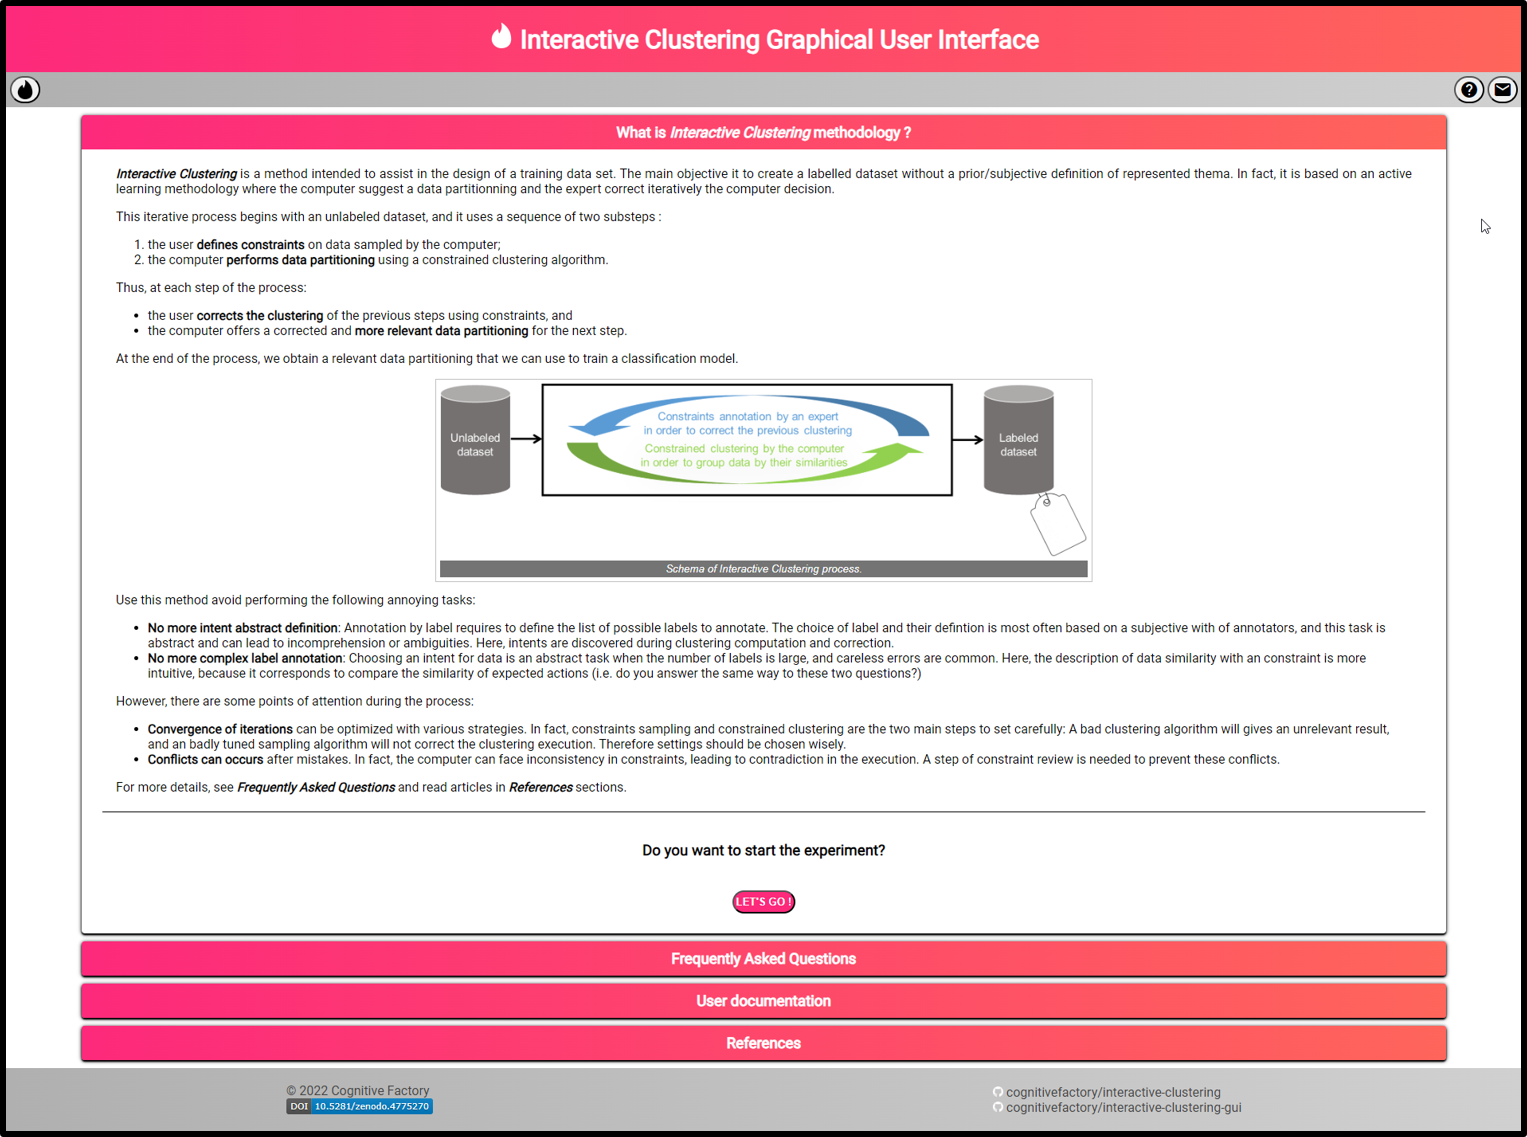
\includegraphics[width=0.95\textwidth]{figures/interactive-clustering-application-accueil-application}
			\caption{
				Capture d'écran de l'application web implémentant notre méthodologie de \texttt{Clustering Interactif} : \textbf{page d'accueil de l'application}.
			}
			\label{figure:C-WEB-APPLICATION-ACCUEIL}
		\end{figure}
		
		% Description générale.
		C'est la page de bienvenu de l'application.
		Nous y trouvons une description rapide de la méthode ainsi qu'une liste des questions fréquentes à son sujet.
		A terme, la documentation de la méthodologie d'annotation y sera intégrée (cf. discussions du \textsc{Chapitre~\ref{chapter:5-GUIDE}}).
		
		% Boutons accessibles.
		Concernant les boutons accessibles :
		\begin{itemize}
			\item Le bouton d'accueil en haut à gauche redirigera toujours sur cette page ;
			\item Le bouton de contact en haut à droite permet de contacter l'équipe de recherche ;
			\item Le bouton \textguillemets{\texttt{LET'S GO}} permet d'accéder à la page de listant les projets d'annotation (cf. \textsc{Figure~\ref{figure:C-WEB-APPLICATION-LISTE-PROJETS}}).
		\end{itemize}
		
		% Information : comme y accéder.
		\begin{leftBarInformation}
			Dans toutes les pages suivantes, il est à noter que :
			\begin{itemize}
				\item Tous les boutons peuvent être survolés pour afficher une courte description de leur action ou de leur état, ainsi que les raccourcis clavier qui permettent de les activer ;
				\item Si besoin, tous les encadrés sont repliables pour gagner en visibilité.
			\end{itemize}
		\end{leftBarInformation}
	
	
	%%% Page de gestion des projets
	\newpage
	\paragraph{Page de gestion des projets (\textsc{Figure~\ref{figure:C-WEB-APPLICATION-LISTE-PROJETS}}) :}
		
		% Capture d'écran: liste des projets.
		\begin{figure}[H]
			\centering
			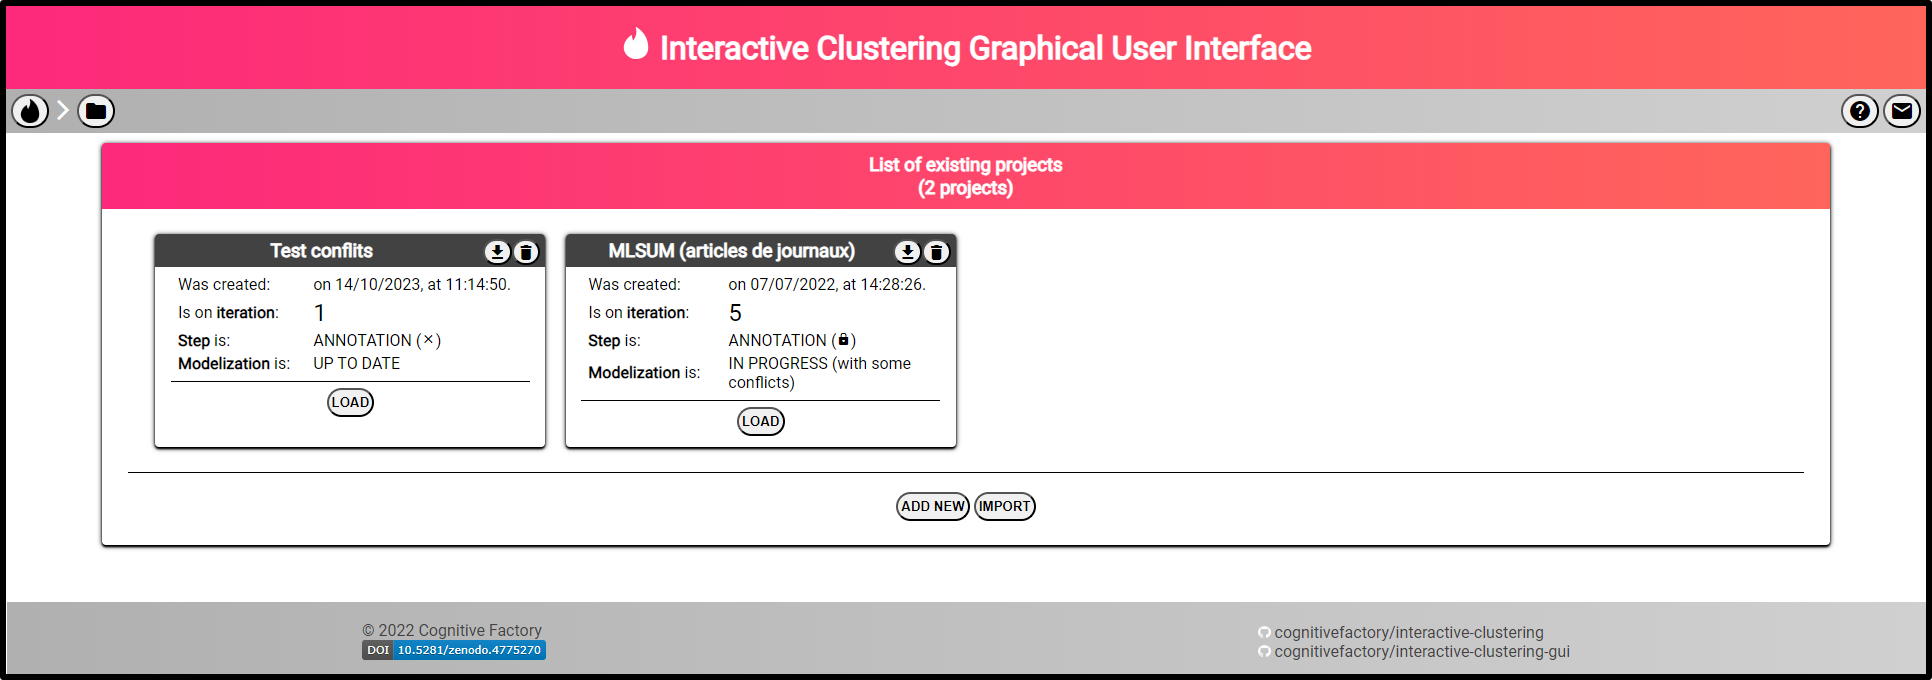
\includegraphics[width=0.95\textwidth]{figures/interactive-clustering-application-liste-projets}
			\caption{
				Capture d'écran de l'application web implémentant notre méthodologie de \texttt{Clustering Interactif} : \textbf{page de gestion des projets}.
			}
			\label{figure:C-WEB-APPLICATION-LISTE-PROJETS}
		\end{figure}
		
		% Description générale.
		Cette page liste les projets existants sous la forme de tuiles contenant les informations importantes : nom, date de création, nombre d'itérations de la méthode, et l'état du projet (cf. \textsc{Figure~\ref{figure:C-WEB-APPLICATION-DIAGRAMME-ETATS}}).
		
		% Boutons accessibles.
		Concernant les boutons d'action de cette page :
		\begin{itemize}
			\item Les boutons d'accueil en haut à gauche permettent de naviguer entre cette page et la page d'accueil de l'application (cf. \textsc{Figure~\ref{figure:C-WEB-APPLICATION-ACCUEIL}}) ;
			\item Il est possible de télécharger un projet au format \texttt{.zip} ou de le supprimer grâce aux boutons \textguillemets{\faDownload} et \textguillemets{\faTrash} en haut à droite de chaque tuile ;
			\item Pour créer un projet, le bouton \textguillemets{\texttt{ADD NEW}} ouvre un formulaire demandant le nom du projet et la liste des textes à annoter (fichier au format \texttt{.csv} avec séparateur '\texttt{;}') ;
			\item Il est aussi possible d'importer un projet contenu dans une archive \texttt{.zip} grâce au bouton \textguillemets{\texttt{IMPORT}} ;
			\item Enfin, le bouton \textguillemets{\texttt{LOAD}} mène à la page d'accueil du projet sélectionné (cf. \textsc{Figure~\ref{figure:C-WEB-APPLICATION-ACCUEIL-PROJET}}).
		\end{itemize}
	
	
	%%% Page d'accueil du projet en cours
	\newpage
	\paragraph{Page d'accueil du projet en cours (\textsc{Figure~\ref{figure:C-WEB-APPLICATION-ACCUEIL-PROJET}}) :}
		
		% Capture d'écran: accueil projet.
		\begin{figure}[H]
			\centering
			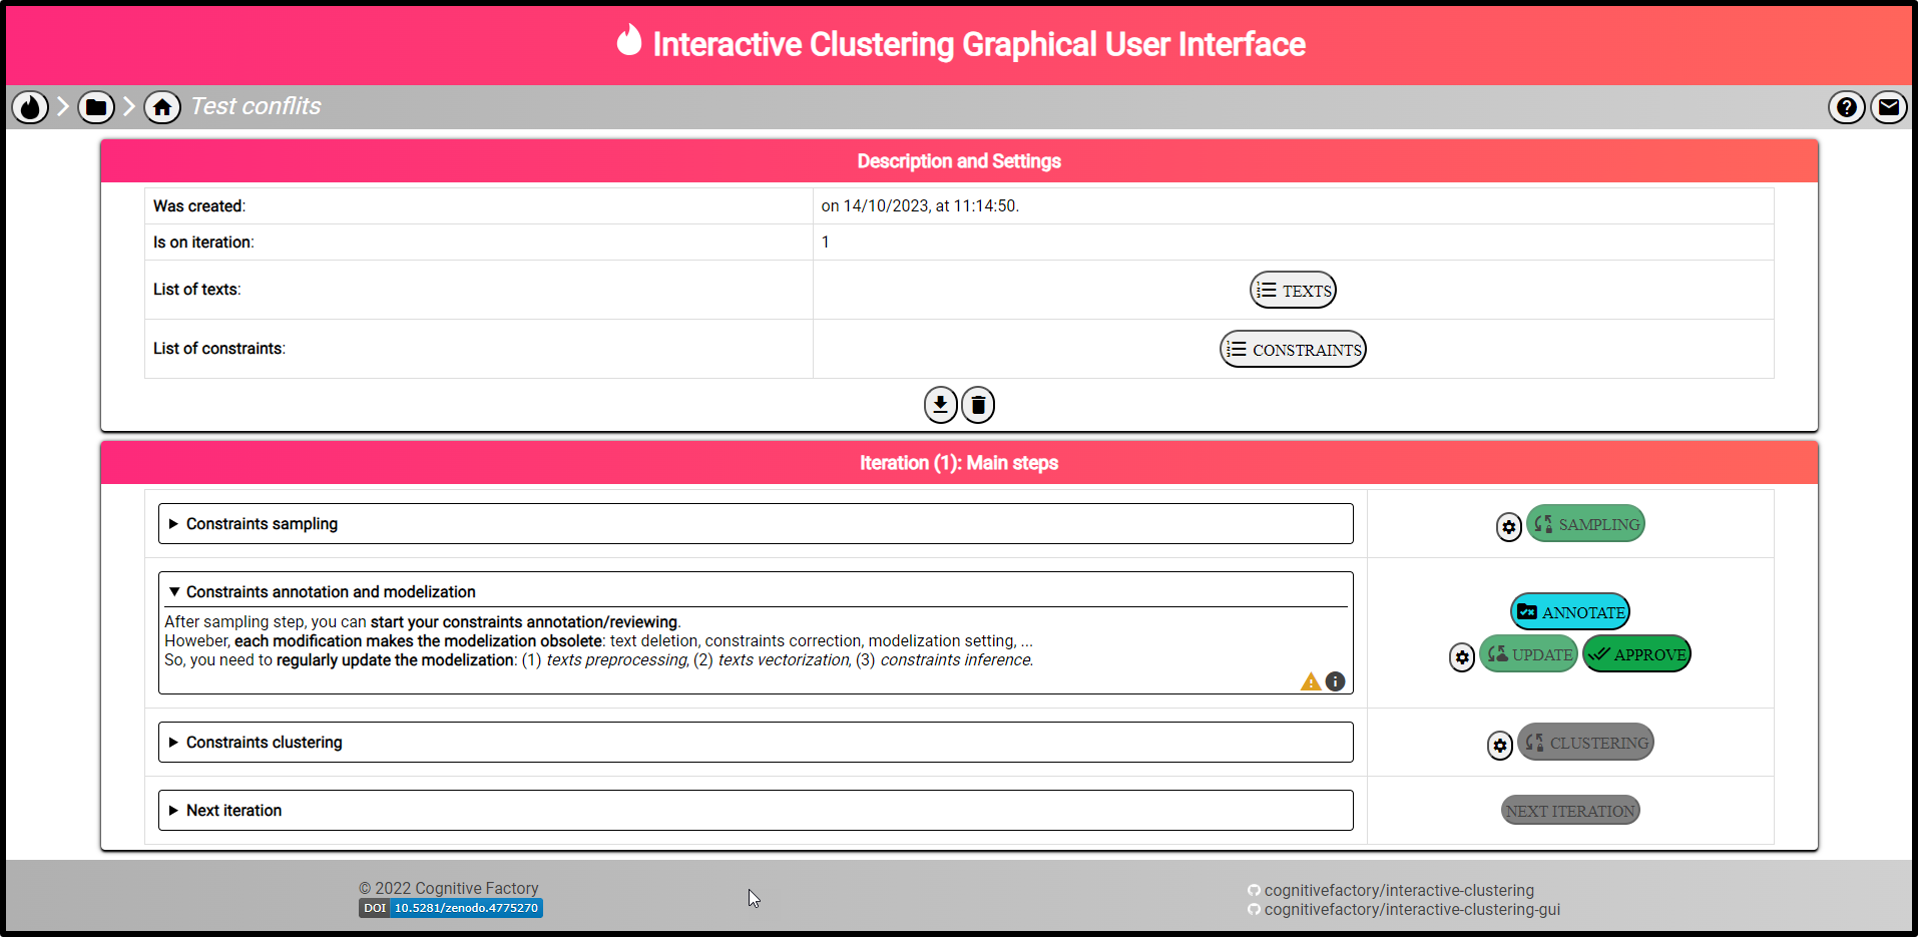
\includegraphics[width=0.95\textwidth]{figures/interactive-clustering-application-accueil-projet}
			\caption{
				Capture d'écran de l'application web implémentant notre méthodologie de \texttt{Clustering Interactif} : \textbf{page d'accueil du projet en cours}.
			}
			\label{figure:C-WEB-APPLICATION-ACCUEIL-PROJET}
		\end{figure}
		
		% Description générale.
		C'est la page principale de l'application.
		Elle contient en partie supérieure les informations du projet d'annotation en cours (\textit{date de création, numéro d'itération, gestion des textes et des contraintes}), et en partie inférieure les étapes d'une itération de \texttt{Clustering Interactif} (\textit{descriptions, boutons d'actions et de paramétrages}).
		
		% Boutons accessibles: gestion de projet.
		Concernant la gestion du projet (partie supérieure) :
		\begin{itemize}
			\item Les boutons d'accueil en haut à gauche permettent de naviguer entre cette page, la page de gestion des projets (cf. \textsc{Figure~\ref{figure:C-WEB-APPLICATION-LISTE-PROJETS}} et la page d'accueil de l'application (cf. \textsc{Figure~\ref{figure:C-WEB-APPLICATION-ACCUEIL}}) ;
			\item Au centre, il est possible de télécharger le projet au format \texttt{.zip} ou de le supprimer grâce aux boutons \textguillemets{\faDownload} et \textguillemets{\faTrash} ;
			\item Le bouton \textguillemets{\texttt{TEXTS}} mène vers la page d'inventaire et de gestion des textes du projet (cf. \textsc{Figure~\ref{figure:C-WEB-APPLICATION-INVENTAIRE-TEXTES}}) ;
			\item Le bouton \textguillemets{\texttt{CONSTRAINTS}} mène vers la page d'inventaire et de gestion des contraintes annotées ou en cours d'annotation (cf. \textsc{Figure~\ref{figure:C-WEB-APPLICATION-INVENTAIRE-CONTRAINTES}}).
		\end{itemize}
		
		% Boutons accessibles: gestion d'une itération.
		Concernant la gestion d'une itération de \texttt{Clustering Interactif} (partie inférieure), les différentes étapes sont représentées de bas en haut à l'aide d'éléments descriptifs repliables et de boutons d'actions.
		Nous retrouvons quatre étapes :
		\begin{enumerate}
			\item l'échantillonnage de contraintes, exécuté en tâche de fond grâce au bouton \textguillemets{\texttt{SAMPLING}}, et dont les paramètres sont accessibles via le bouton \textguillemets{\faCog} ;
			\item l'annotation de contraintes, avec le bouton \textguillemets{\texttt{ANNOTATE}} qui redirige vers la prochaine contrainte à annoter.
			Cette étape contient aussi une gestion de la modélisation, c'est-à-dire une vérification des prétraitements et de la vectorisation des textes, ainsi qu'une vérification de la cohérence des contraintes par l'absence de conflits d'annotation : le bouton \textguillemets{\texttt{UPDATE}} permet de recalculer cette modélisation en tâche de fond et le bouton \textguillemets{\texttt{APPROVE}} permet de la fixer jusqu'à la fin de l'itération en cours ;
			\item l'\textit{clustering} sous contraintes, exécuté en tâche de fond grâce au bouton \textguillemets{\texttt{CLUSTERING}}, et dont les paramètres sont accessibles via le bouton \textguillemets{\faCog} ;
			\item la confirmation du passage à la nouvelle itération, exécutée grâce au bouton \textguillemets{\texttt{NEXT ITERATION}}.
		\end{enumerate}
		
		% Notes:
		Il est à noter que :
		\begin{itemize}
			\item Les éléments de gauche sont repliables : au chargement de la page, seul l'élément de l'étape en cours est déplié ;
			\item La gestion de l'itération se fait à l'aide d'un diagramme d'état (cf. \textsc{Figure~\ref{figure:C-WEB-APPLICATION-DIAGRAMME-ETATS}}) : celui-ci se manifeste par un code couleur et l'activation/désactivation des boutons.
		\end{itemize}
	
	
	%%% Diagramme d'états de l'application et gestion des exécutions asynchrones
	\newpage
	\paragraph{Diagramme d'états de l'application et gestion des exécutions asynchrones (\textsc{Figure~\ref{figure:C-WEB-APPLICATION-DIAGRAMME-ETATS}}) :}
		
		% Capture d'écran: accueil projet.
		\begin{figure}[H]
			\centering
			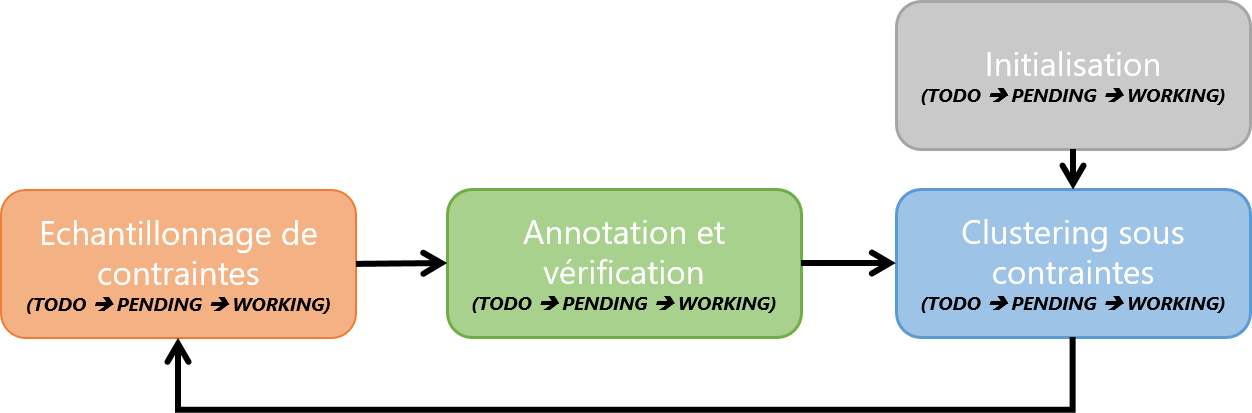
\includegraphics[width=0.95\textwidth]{figures/interactive-clustering-application-diagramme-etats}
			\caption{
				\textbf{Diagramme d'états} simplifié de l'application web implémentant notre méthodologie de \texttt{Clustering Interactif}.
			}
			\label{figure:C-WEB-APPLICATION-DIAGRAMME-ETATS}
		\end{figure}
		
		% Description générale.
		Comme décrit en \textsc{Section~\ref{section:3.2-DESCRIPTION-THEORIQUE}} et dans la \textsc{Figure~\ref{figure:3.2.1-DESCRIPTION-THEORIQUE-GENERALE}}, une itération de \textit{Clustering Interactif} contient trois étapes majeures : \textbf{(1)} l'échantillonnage de contraintes, \textbf{(2)} l'annotation de contraintes, et \textbf{(3)} le \textit{clustering} sous contraintes.
		Ces étapes sont représentées par le diagramme d'état en \textsc{Figure~\ref{figure:C-WEB-APPLICATION-DIAGRAMME-ETATS}} : ce dernier définit l'activation ou la désactivation des boutons d'action de l'application (cf. \textsc{Figure~\ref{figure:C-WEB-APPLICATION-ACCUEIL-PROJET}}).
		
		% Gestion de couleur.
		Afin de représenter l'état en cours et les actions possibles de manière pragmatique dans l'interface, un code couleur implicite est utilisé en plus de l'activation/désactivation des boutons :
		\begin{itemize}
			\item objet \textguillemets{\textcolor{colorApplicationNOTAVAILABLE}{\textbf{grisé}}} et généralement désactivé : action inaccessible pour le moment ;
			\item objet en \textguillemets{\textcolor{colorApplicationAVAILABLE}{\textbf{vert}}} et activé : prochaine action à réaliser ;
			\item objet en \textguillemets{\textcolor{colorApplicationWORKING}{\textbf{cyan}}} : action en cours de traitement ;
			\item objet en \textguillemets{\textcolor{colorApplicationERROR}{\textbf{rouge}}} et activé : action en erreur ou à recommencer ;
			\item objet en \textguillemets{\textcolor{colorApplicationDONE}{\textbf{vert grisé}}} et généralement désactivé : action réalisée avec succès.
		\end{itemize}
		
		% Gestion des actions asynchrones.
		D'autre part, comme certains algorithmes peuvent être lents, ces derniers sont exécutés en tâche de fond.
		La gestion d'état est alors affinée en quatre sous-états :
		\begin{itemize}
			\item \textguillemets{\textcolor{colorApplicationAVAILABLE}{\textbf{\texttt{TODO}}}} : l'action est à faire, la machine attend l'ordre de l'utilisateur ;
			\item \textguillemets{\textcolor{colorApplicationWORKING}{\textbf{\texttt{PENDING}}}} : l'action a été ordonnée par l'utilisateur, mais elle n'a pas encore été prise en charge par la machine ;
			\item \textguillemets{\textcolor{colorApplicationWORKING}{\textbf{\texttt{WORKING}}}} : l'action est en cours d'exécution en tâche de fond.
			Une barre d'avancement apparaît pour maintenir l'utilisateur informé de l'évolution de cet état ;
			\item \textit{Note} : l'état \textguillemets{\textcolor{colorApplicationDONE}{\textbf{\texttt{DONE}}}} (action faite) n'existe pas réellement, elle est représentée par le fait que la prochaine étape ait un état \textguillemets{\texttt{TODO}}.
		\end{itemize}
		
		% Warning: Architecture asynchrone en production.
		\begin{leftBarWarning}
			Pour une simplicité d'usage et afin d'offrir une démonstration rapide de notre méthodologie, nous avons décidé d'exécuter simplement les algorithmes en tâche de fond.
			Toutefois, pour favoriser les performances de l'application ainsi que sa sûreté pour une utilisation en production, nous vous conseillons de ré-implémenter cette gestion des exécutions en privilégiant une architecture asynchrone utilisant des \textit{workers} dédiés.
		\end{leftBarWarning}
	
	
	%%% Page de gestion des paramètres
	\newpage
	\paragraph{Page de gestion des paramètres (\textsc{Figure~\ref{figure:C-WEB-APPLICATION-PARAMETRAGE}}) :}
	
		% Capture d'écran: gestion des paramètrages.
		\begin{figure}[H]
			\centering
			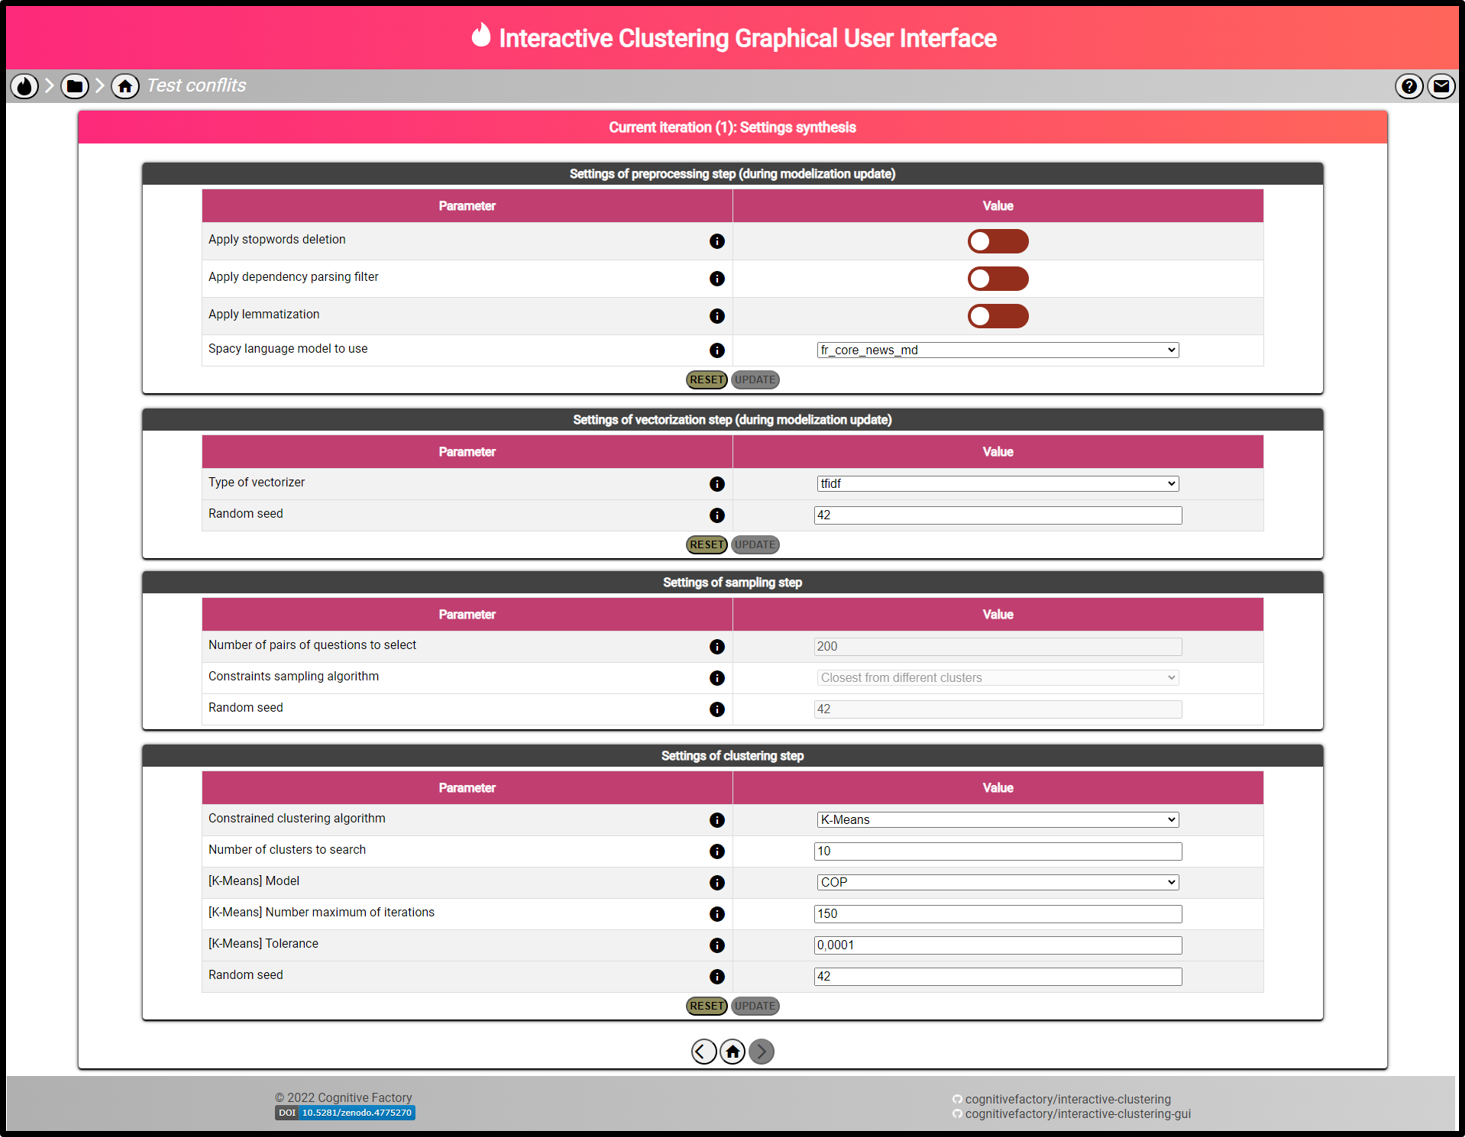
\includegraphics[width=0.95\textwidth]{figures/interactive-clustering-application-parametres}
			\caption{
				Capture d'écran de l'application web implémentant notre méthodologie de \texttt{Clustering Interactif} : \textbf{page de gestion des paramètres}.
			}
			\label{figure:C-WEB-APPLICATION-PARAMETRAGE}
		\end{figure}
		
		% Description générale.
		Accessible depuis les différents boutons \textguillemets{\faCog}, cette page liste les divers paramètres des algorithmes pour chaque itération.
		\begin{itemize}
			\item Chaque tuile représente une tâche (prétraitements, vectorisation, échantillonnage et \textit{clustering}) : divers algorithmes et hyperparamètres son disponibles ;
			\item Les boutons \textguillemets{\texttt{UPDATE}} permettent de valider les changements, les boutons \textguillemets{\texttt{RESET}} rétablissent les paramètres par défaut ;
			\item Ces différents formulaires sont modifiables tant que l'étape n'est pas en cours d'exécution, sinon ils sont juste consultables ;
			\item En bas de page, il est possible de changer d'itération pour consulter les paramètres des itérations précédentes (boutons \textguillemets{\faAngleLeft} et \textguillemets{\faAngleRight}), et de revenir vers la page d'accueil du projet (bouton \textguillemets{\faHome}, cf. \textsc{Figure~\ref{figure:C-WEB-APPLICATION-ACCUEIL-PROJET}}).
		\end{itemize}
	
	
	%%% Page d'inventaire des textes
	\newpage
	\paragraph{Page d'inventaire des textes (\textsc{Figure~\ref{figure:C-WEB-APPLICATION-INVENTAIRE-TEXTES}}) :}
	
		% Capture d'écran: inventaire des textes.
		\begin{figure}[H]
			\centering
			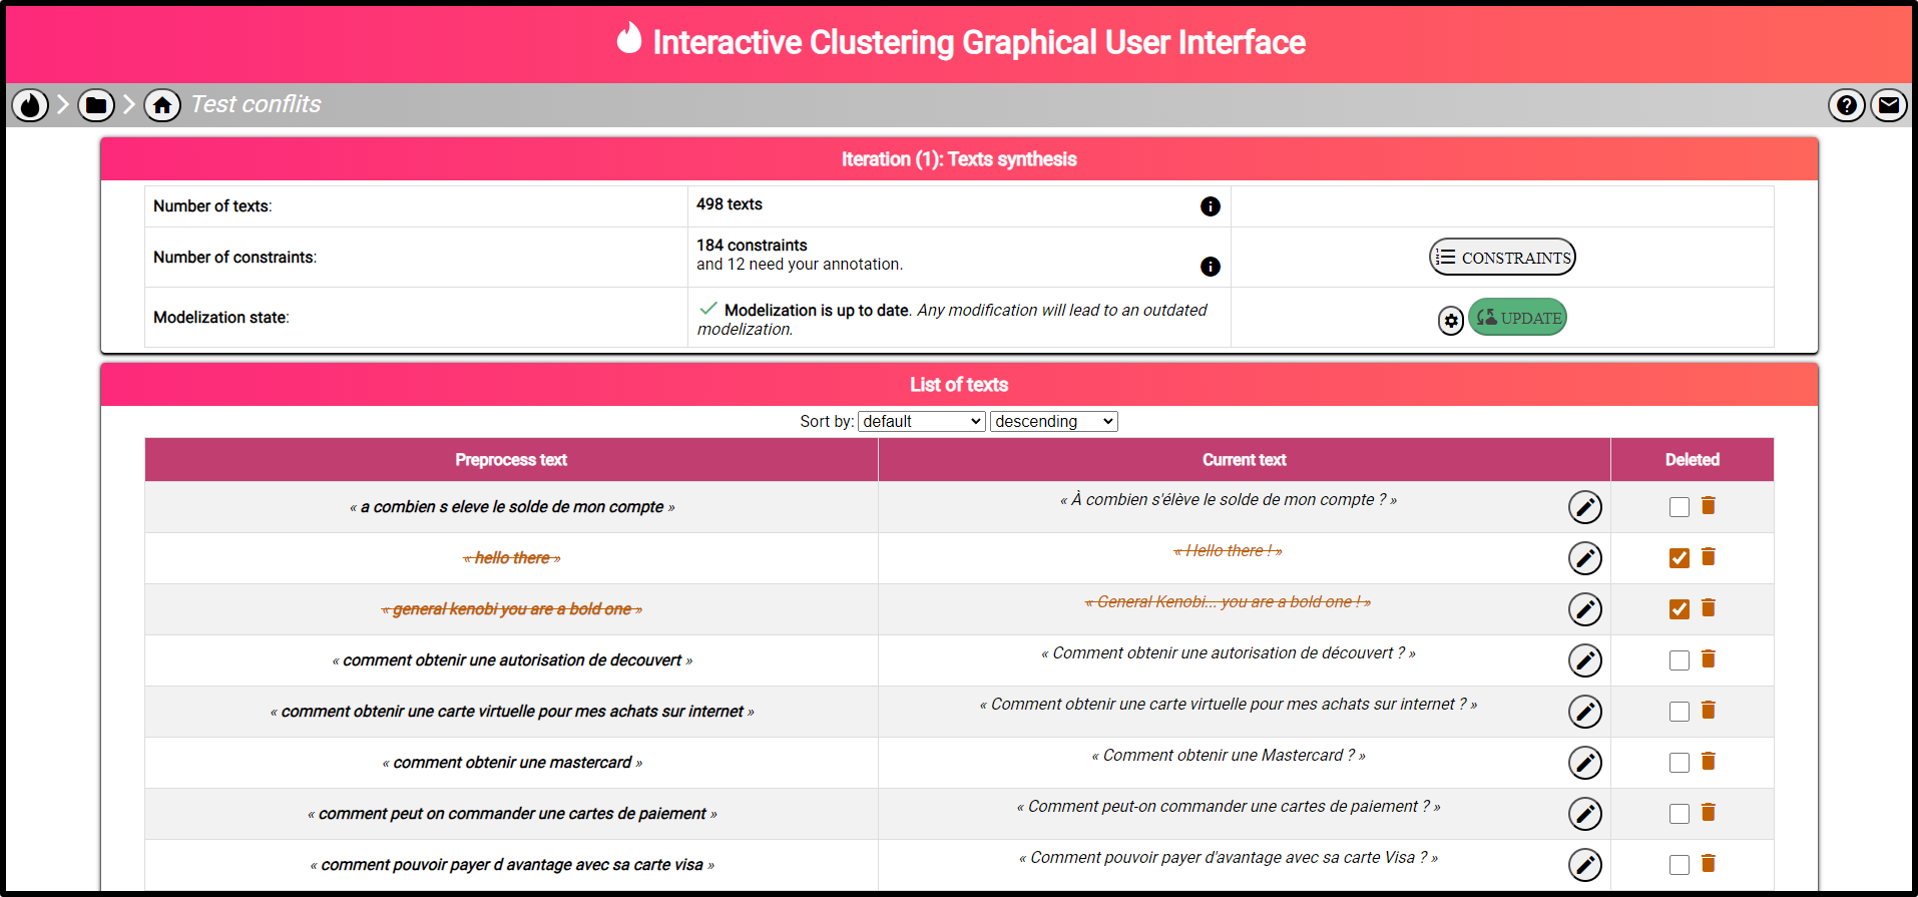
\includegraphics[width=0.95\textwidth]{figures/interactive-clustering-application-textes}
			\caption{
				Capture d'écran de l'application web implémentant notre méthodologie de \texttt{Clustering Interactif} : \textbf{page d'inventaire des textes}.
			}
			\label{figure:C-WEB-APPLICATION-INVENTAIRE-TEXTES}
		\end{figure}
		
		% Description générale.
		Cette page permet de lister les textes du projet à annoter.
		La page est divisée en deux : la partie supérieure donne des informations générales (\textit{nombre de textes, nombre de contraintes à annoter, rappel de la modélisation en cours}), et la partie inférieure liste les textes dans un tableau.
		
		% Boutons accessibles: gestion des textes.
		Concernant les informations générales (partie supérieure) :
		\begin{itemize}
			\item Le bouton \textguillemets{\texttt{UPDATE}} permet de mettre à jour la modélisation si des contraintes ont été ajoutées, des paramètres de prétraitements ou de vectorisation ont été mis à jour, ou si des textes ont été modifiés : cette action est exécutée en tâche de fond.
			La couleur de se bouton est définie par le diagramme d'état (cf. \textsc{Figure~\ref{figure:C-WEB-APPLICATION-DIAGRAMME-ETATS}}) ;
			\item Le bouton \textguillemets{\texttt{CONSTRAINTS}} mène vers la page d'inventaire et de gestion des contraintes annotées ou en cours d'annotation (cf. \textsc{Figure~\ref{figure:C-WEB-APPLICATION-INVENTAIRE-CONTRAINTES}}).
		\end{itemize}
		
		% Boutons accessibles: liste des textes.
		Concernant le tableau listant les textes (partie inférieure) :
		\begin{itemize}
			\item Le texte brut et sa version prétraitée sont affichés ;
			\item Grâce au bouton \textguillemets{\faPen}, il est possible de corriger un texte s'il contient une faute de frappe ;
			\item Grâce au bouton \textguillemets{\textcolor{colorApplicationDELETE}{\faTrash}}, il est possible de supprimer (\textit{ne plus prendre en compte}) un texte s'il n'est pas pertinent pour le projet : celui-ci est alors rayé en \textcolor{colorApplicationDELETE}{orange} ;
			\item En haut du tableau, il est possible de trier les textes suivant différents critères (\textit{ordre alphabétique, supprimé ou non, ...}) ;
			\item \textbf{Attention} : Toute action de modification (renommage, suppression) nécessite de mettre à jour la modélisation par la suite.
			De plus, ces actions sont désactivées si le projet n'est pas à l'étape d'annotation (cf. diagramme d'états en \textsc{Figure~\ref{figure:C-WEB-APPLICATION-DIAGRAMME-ETATS}}) ;
		\end{itemize}
	
	
	%%% Page d'inventaire des contraintes
	\newpage
	\paragraph{Page d'inventaire des contraintes (\textsc{Figure~\ref{figure:C-WEB-APPLICATION-INVENTAIRE-CONTRAINTES}}) :}
	
		% Capture d'écran: inventaire des contraintes.
		\begin{figure}[H]
			\centering
			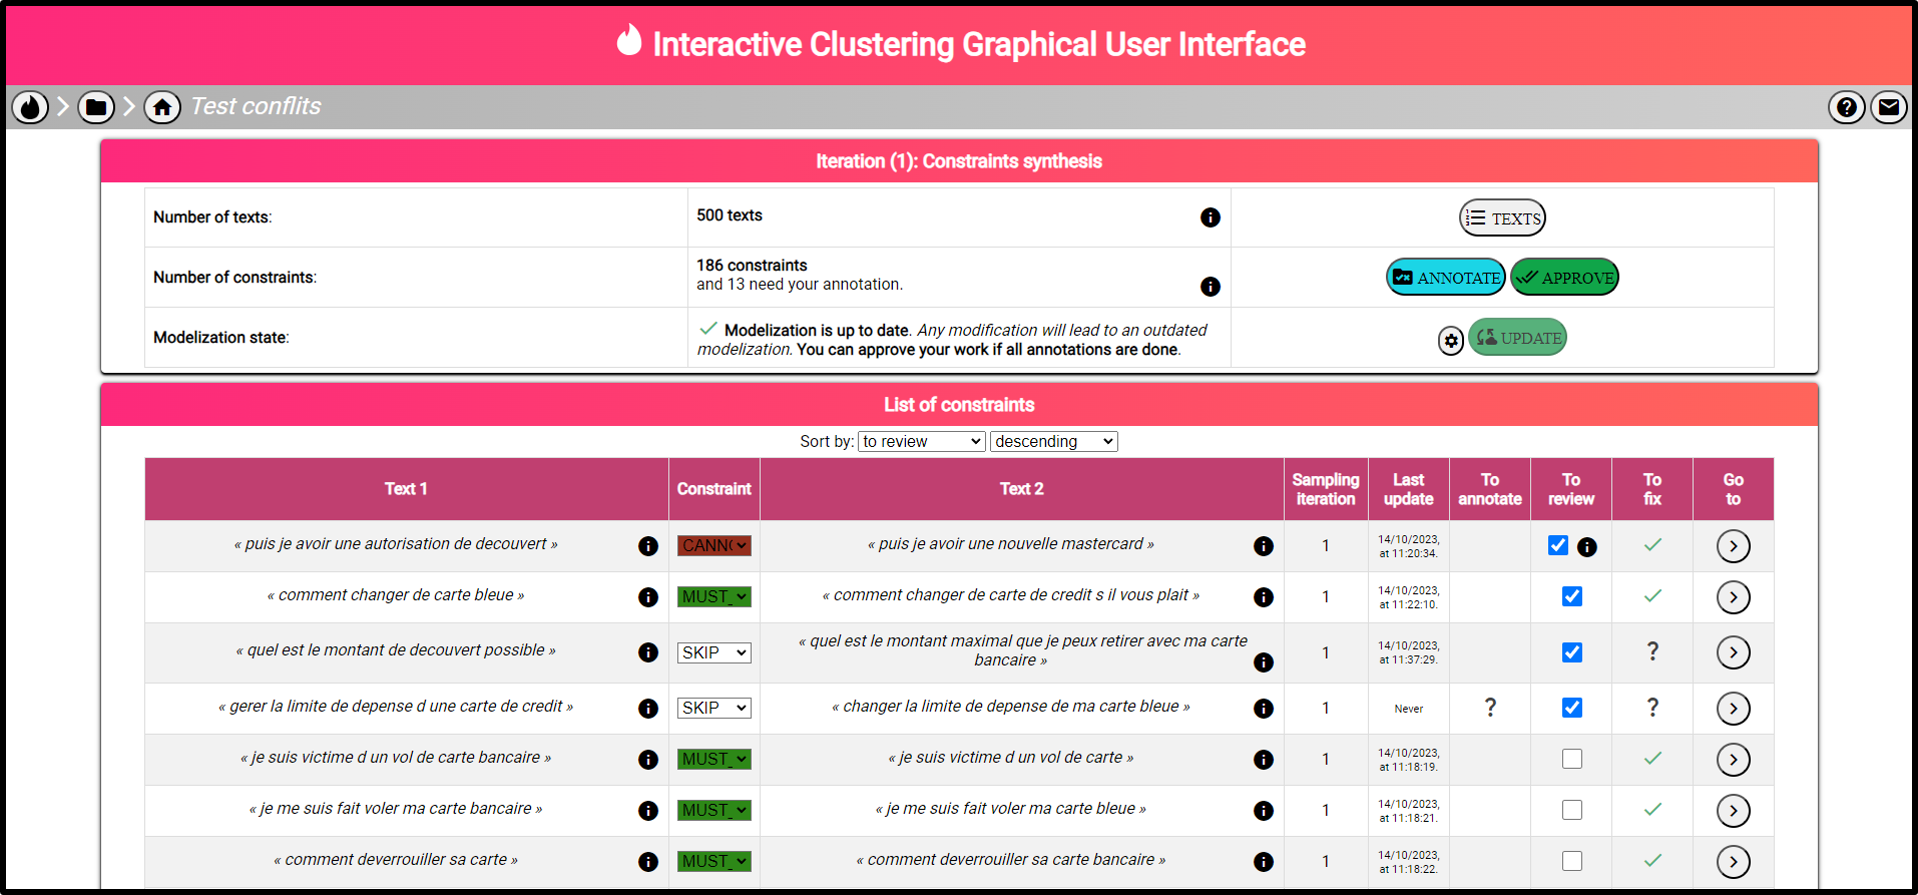
\includegraphics[width=0.95\textwidth]{figures/interactive-clustering-application-contraintes}
			\caption{
				Capture d'écran de l'application web implémentant notre méthodologie de \texttt{Clustering Interactif} : \textbf{page d'inventaire des contraintes}.
			}
			\label{figure:C-WEB-APPLICATION-INVENTAIRE-CONTRAINTES}
		\end{figure}
		
		% Description générale.
		Cette page permet de lister les contraintes du projet à annoter.
		La page est divisée en deux : la partie supérieure donne des informations générales (\textit{nombre de textes, nombre des contraintes à annoter, rappel de la modélisation en cours}), et la partie inférieure liste les contraintes dans un tableau.
		
		% Boutons accessibles: gestion des contraintes.
		Concernant les informations générales (partie supérieure) :
		\begin{itemize}
			\item Le bouton \textguillemets{\texttt{ANNOTATE}} redirige vers la prochaine contrainte à annoter (s'il en reste) ;
			\item Le bouton \textguillemets{\texttt{UPDATE}} permet de mettre à jour la modélisation si des contraintes ont été ajoutées, des paramètres de prétraitements ou de vectorisation ont été mis à jour, ou si des textes ont été modifiés : cette action est exécutée en tâche de fond.
			La couleur de se bouton est définie par le diagramme d'état (cf. \textsc{Figure~\ref{figure:C-WEB-APPLICATION-DIAGRAMME-ETATS}}) ;
			\item Le bouton \textguillemets{\texttt{TEXTS}} mène vers la page d'inventaire et de gestion des données du projet (cf. \textsc{Figure~\ref{figure:C-WEB-APPLICATION-INVENTAIRE-TEXTES}}).
		\end{itemize}
		
		% Boutons accessibles: liste des contraintes.
		Concernant le tableau listant les contraintes (partie inférieure) :
		\begin{itemize}
			\item Les deux textes d'une même contrainte sont affichés de part et d'autre de la valeur annotée : \textcolor{colorApplicationMUSTLINK}{\texttt{MUST-LINK}}, \textcolor{colorApplicationCANNOTLINK}{\texttt{CANNOT-LINK}} ou \texttt{SKIP} (\textit{pour une contrainte non-annotée ou temporairement ignorée}) ;
			\item Il est possible de marquer une contrainte pour la revoir plus tard grâce à la coche \textguillemets{\textcolor{colorApplicationREVIEW}{\faCheckSquare}} ;
			\item Le bouton \textguillemets{\faAngleRight} à droite permet d'accéder à la page d'annotation de cette contrainte (cf. \textsc{Figure~\ref{figure:C-WEB-APPLICATION-ANNOTATION}}) ;
			\item Diverses informations sont disponibles à la droite du tableau : l'itération à laquelle la contrainte a été échantillonnée, sa dernière date de modification, son besoin d'annotation (\textit{\textguillemets{\faQuestion} pour une contrainte encore jamais été annotée}), et la présence ou non de conflits (\textit{\textguillemets{\textcolor{colorApplicationMUSTLINK}{\faCheck}} ou \textguillemets{\textcolor{colorApplicationERROR}{\faExclamation}}}) ;
			\item En haut du tableau, il est possible de trier les contraintes suivant différents critères (\textit{ordre alphabétique, valeur d'annotation, date d'échantillonnage ou de modification, présence de conflit, ...}) ;
			\item \textbf{Attention} : Toute action de modification de la valeur d'annotation nécessite de mettre à jour la modélisation par la suite ;
			De plus, cette action est désactivée si le projet n'est pas à l'étape d'annotation (cf. diagramme d'états en \textsc{Figure~\ref{figure:C-WEB-APPLICATION-DIAGRAMME-ETATS}}) ;
			\item \textit{Note} : Si une contrainte concerne au moins un texte qui a été supprimé (cf. \textsc{Figure~\ref{figure:C-WEB-APPLICATION-INVENTAIRE-TEXTES}}), la contrainte n'apparaît pas dans ce tableau mais existe toujours dans l'application (\textit{elle n'est plus prise en compte}).
		\end{itemize}
	
	
	%%% Page d'annotation d'une contrainte
	\newpage
	\paragraph{Page d'annotation d'une contrainte (\textsc{Figure~\ref{figure:C-WEB-APPLICATION-ANNOTATION}} et \textsc{Figure~\ref{figure:C-WEB-APPLICATION-CONFLIT}}) :}
	
		% Capture d'écran: annotation.
		\begin{figure}[H]
			\centering
			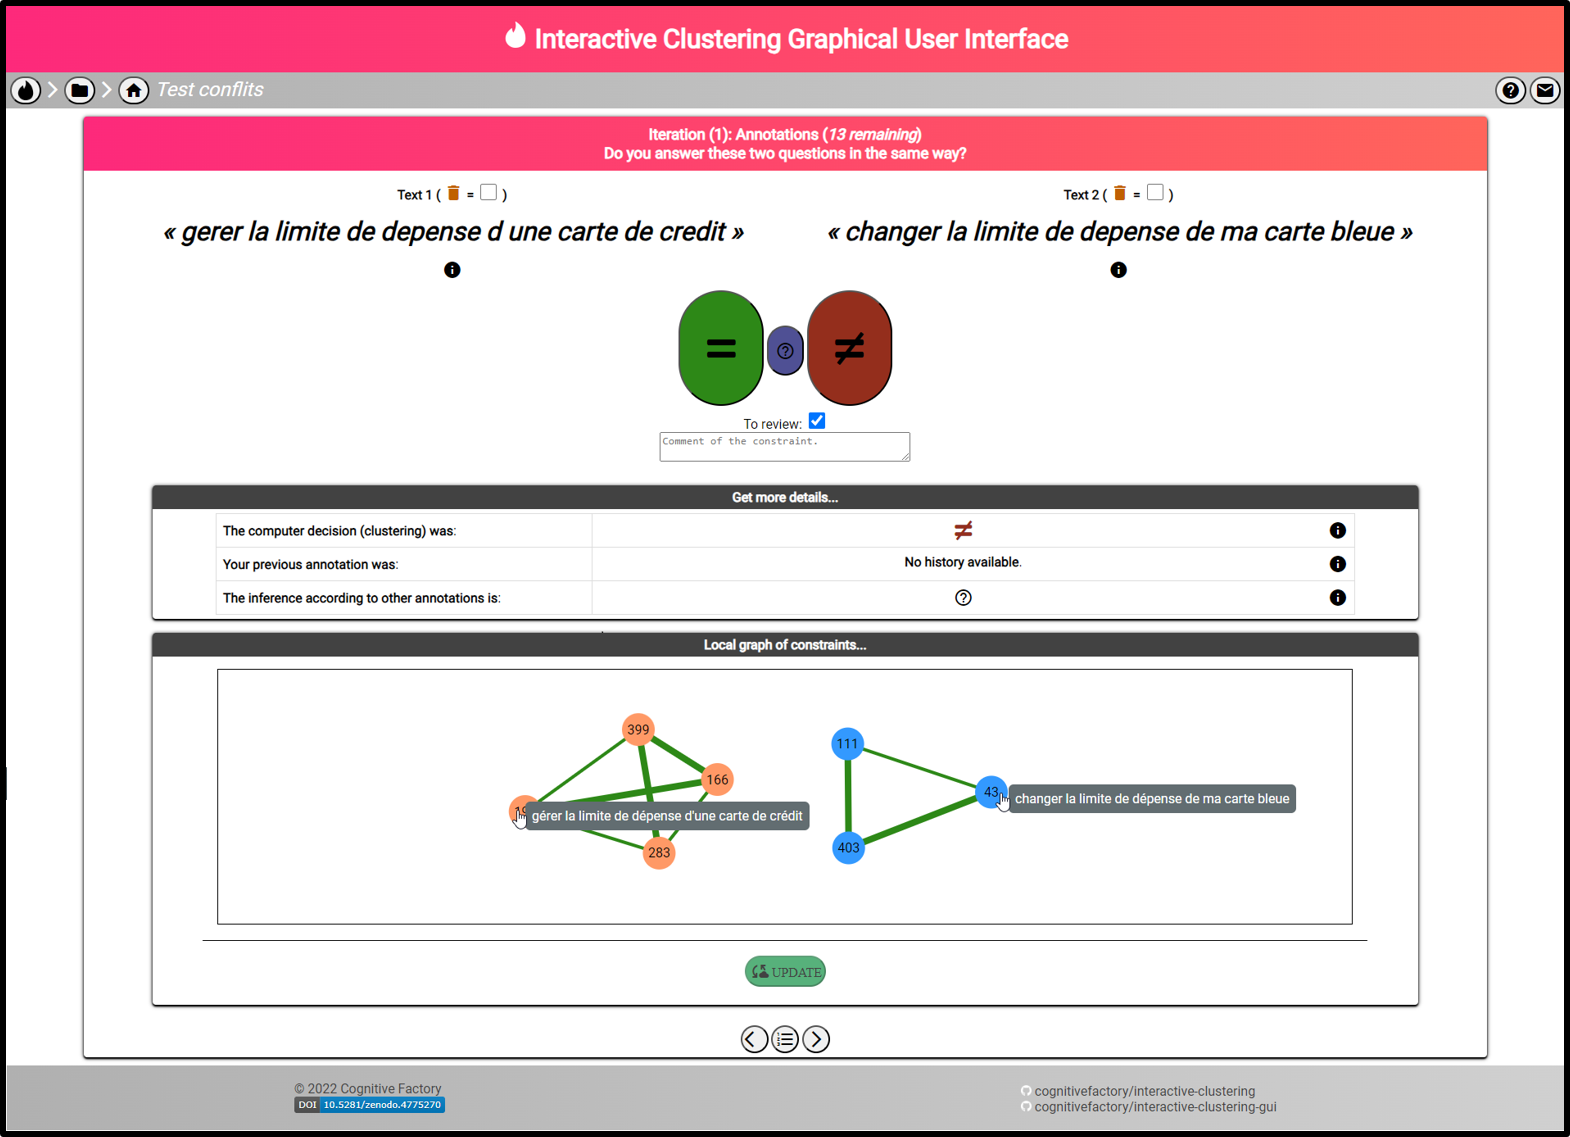
\includegraphics[width=0.95\textwidth]{figures/interactive-clustering-application-annotation-0full}
			\caption{
				Capture d'écran de l'application web implémentant notre méthodologie de \texttt{Clustering Interactif} : \textbf{page d'annotation d'une contrainte}.
			}
			\label{figure:C-WEB-APPLICATION-ANNOTATION}
		\end{figure}
		
		% Description générale.
		Cette page est le coeur de cette application d'annotation : la partie supérieure permet d'annoter une contraintes entre deux textes, les parties inférieures sont des détails (éléments repliés par défaut).
		
		% Boutons accessibles: annotation.
		Concernant l'annotation de la contrainte (partie supérieure) :
		\begin{itemize}
			\item Les deux textes de la contrainte sont affichés en haut du bloc d'annotation ;
			\item Les deux boutons principaux d'annotation sont le \textguillemets{\textcolor{colorApplicationMUSTLINK}{\faEquals}} pour un \texttt{MUST-LINK} et le \textguillemets{\textcolor{colorApplicationCANNOTLINK}{\faNotEqual}} pour un \texttt{CANNOT-LINK}.
			Les raccourcis claviers de ses boutons sont respectivement \textguillemets{\texttt{A}} (\textit{accept}) et \textguillemets{\texttt{R}} (\textit{reject}).
			Il est aussi possible d'ignorer la contrainte avec le bouton \textguillemets{\textcolor{colorApplicationSKIP}{\faQuestion}} (raccourcis avec la barre espace) ;
			\item Si c'est la première fois que cette contrainte est annotée, la prochaine contrainte est automatiquement chargée lors d'un choix d'annotation (\textguillemets{\textcolor{colorApplicationMUSTLINK}{\faEquals}}, \textguillemets{\textcolor{colorApplicationCANNOTLINK}{\faNotEqual}} ou \textguillemets{\textcolor{colorApplicationSKIP}{\faQuestion}}).
			Sinon, une confirmation est demandée pour valider le changement de la valeur de la contrainte ;
			\item Une gestion de revue d'annotation est possible grâce à un champ de commentaire, et \textguillemets{\textcolor{colorApplicationREVIEW}{\faCheckSquare}} permet de marquer la contrainte pour la pour revoir plus tard ;
			\item Grâce à l'icône info-bulle, il est possible d'afficher la version non-prétraitée de chaque texte
			De plus, grâce à la coche \textguillemets{\textcolor{colorApplicationDELETE}{\faTrash}}, il est possible de supprimer (\textit{ne plus prendre en compte}) un texte non pertinent pour le projet : la contrainte sera alors masquée de la liste des contraintes ;
			\item \textbf{Attention} : Toute action de modification de la valeur d'annotation nécessite de mettre à jour la modélisation par la suite.
			De plus, cette action est désactivée si le projet n'est pas à l'étape d'annotation (cf. diagramme d'états en \textsc{Figure~\ref{figure:C-WEB-APPLICATION-DIAGRAMME-ETATS}}) ;
		\end{itemize}
		
		% Boutons accessibles: détails.
		Concernant les détails sur la contraintes (partie inférieure) :
		\begin{itemize}
			\item L'encadré du milieu donne quelques informations sur l'annotation : ce qu'a effectué la machine lors de la précédente étape de \textit{clustering} (même \textit{cluster} ou différentes \textit{clusters} ?), l'historique de ce que l'annotateur a renseigné au préalable, et la déduction faite par le gestionnaire de contraintes grâce aux propriétés de transitivité ;
			\item L'encadré du bas propose une visualisation du graphe de contraintes à l'aide de la librairie \texttt{d3js} \footnote {
				\url{https://d3js.org/}
			} ;
			\item Les boutons en bas de page permettent de naviguer entre les pages d'annotation (boutons \textguillemets{\faAngleLeft} et \textguillemets{\faAngleRight}) ou à revenir vers la page d'inventaire des contraintes (bouton \textguillemets{\faList}, cf. \textsc{Figure~\ref{figure:C-WEB-APPLICATION-INVENTAIRE-CONTRAINTES}}).
		\end{itemize}
		
		% Capture d'écran: conflit d'annotation.
		\begin{figure}[H]
			\centering
			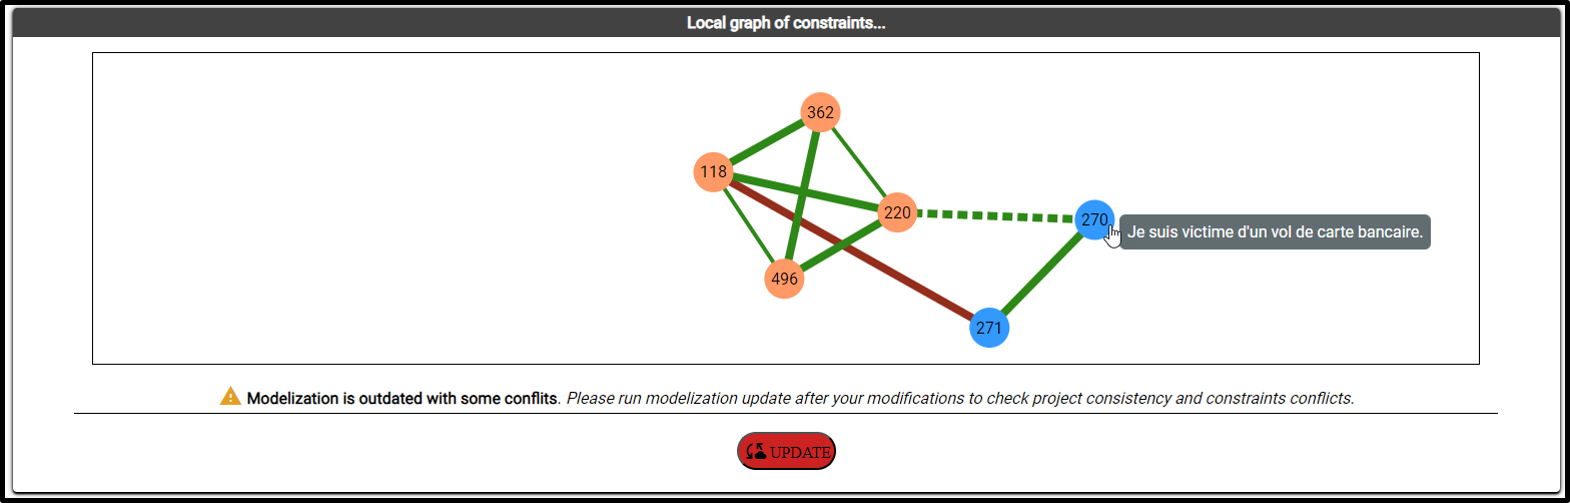
\includegraphics[width=0.95\textwidth]{figures/interactive-clustering-application-annotation-4conflit}
			\caption{
				Capture d'écran de l'application web implémentant notre méthodologie de \texttt{Clustering Interactif} : \textbf{graphe de contraintes présentant un conflit d'annotation}.
			}
			\label{figure:C-WEB-APPLICATION-CONFLIT}
		\end{figure}
		
		% Graphe de contraintes.
		Concernant le graphe local de contraintes :
		\begin{itemize}
			\item Les cercles représentent les données : chaque numéro correspond à un identifiant, et leurs textes respectifs sont visibles par un survol de souris.
			Ces cercles peuvent être déplacés pour une meilleur visibilité ;
			\item Les liens entre les cercles représentent les contraintes : en \textcolor{colorApplicationMUSTLINK}{\textbf{vert}} pour les \texttt{MUST-LINK} et en \textcolor{colorApplicationCANNOTLINK}{\textbf{rouge}} pour les \texttt{CANNOT-LINK}, en \textbf{gras} pour les contraintes annotées et en \textit{fin} pour les contraintes déduites par transitivité, et en \texttt{pointillés} pour les conflits détectés.
			Un clic de souris sur un lien redirige vers la page d'annotation de la contrainte associée (si elle existe) ;
			\item Comme il peut y avoir un nombre important de contraintes dans un projet, ce graphe ne représente que la partie des contraintes impliquées dans l'annotation des deux textes de cette page : on retrouve ainsi les deux textes en cours d'annotation et leurs composants connexes respectifs (voir \textsc{Section~\ref{annex:C.1.2-DESCRIPTION-IMPLEMENTATION-INTERACTIVE-CLUSTERING-GESTION-DES-CONTRAINTES}}) ;
			\item Dans l'exemple en \textsc{Figure~\ref{figure:C-WEB-APPLICATION-CONFLIT}}, on peut voir le conflit suivant : \textbf{(1)} $118$ et $270$ doivent être séparés car $118$ est différent de $271$ qui est similaire à $270$, mais \textbf{(2)} $118$ et $270$ doivent être rapprochés car $118$ est similaire à $220$ qui est similaire à $270$...
			\item \textbf{Attention} : En cas de conflit, plusieurs boutons deviennent \textcolor{colorApplicationERROR}{\textbf{rouge}}, et l'approbation de la modélisation est désactivée tant que le conflit n'est pas résolu.
		\end{itemize}
	
	
	%%%%%--------------------------------------------------------------------
	%%%%% Section C.3: Implémentation de la librairie \texttt{cognitivefactory-interactive-clustering}
	%%%%%--------------------------------------------------------------------
	\newpage
	\section[
		\texttt{cognitivefactory-features-maximization-metric}
	]{
		Implémentation de l'application web \\ \texttt{cognitivefactory-features-maximization-metric}
	}
\label{annex:C.3-DESCRIPTION-IMPLEMENTATION-FEATURES-MAXIMIZATION-METRIC}
	
	% Généralités.
	La librairie \texttt{cognitivefactory-features-maximization-metric} (\cite{schild:2023:cognitivefactory-featuresmaximizationmetric}) ...
	\todo[inline]{introduction à rédiger}
	
	% Information : comme y accéder.
	\begin{leftBarInformation}
		La documentation technique est accessible au lien suivant : \url{https://cognitivefactory.github.io/features-maximization-metric/}.
	\end{leftBarInformation}